\documentclass[print, color, oneside]{ugrTFG}
\usepackage{url}           % Para poder manejar enlaces URL correctamente
\usepackage[utf8]{inputenc}
\usepackage{amsmath}       % Si usas matemáticas
\usepackage{geometry}
\usepackage{tcolorbox}
\usepackage{listings}
\usepackage{csquotes}
\usepackage{placeins}
\usepackage{float}
\usepackage{makecell} 
\usepackage[perpage]{footmisc} % Reinicia la numeración en cada página
\usepackage[backend=biber,style=numeric,sorting=none]{biblatex}
\addbibresource{../capitulos/referencias.bib}
\geometry{twoside=false}
\geometry{left=2.5cm, right=2.5cm, top=3cm, bottom=3cm}

\lstset{
    breaklines=false,   % Evita que las líneas se corten
    prebreak={},        % Evita cortes de línea innecesarios
    xleftmargin=-2.2cm,   % Desplaza el código a la izquierda
    numbers=none,       % Quita la numeración de líneas
    frame=none          % Quita el recuadro alrededor del código
}

% -------------------------------------------------------------------
% INFORMACIÓN DEL TFG Y EL AUTOR
% -------------------------------------------------------------------

\newcommand{\miTitulo}{Metodologías Multivariantes para la Identificación de Patrones Biológicos\xspace}
\newcommand{\miNombre}{Quintín Mesa Romero\xspace}
\newcommand{\miGrado}{Doble Grado en Ingeniería Informática y Matemáticas}
\newcommand{\miFacultad}{Facultad de Ciencias}
\newcommand{\miFacultadBis}{E.T.S. Ingenierías Informática y de Telecomunicación}
\newcommand{\miUniversidad}{Universidad de Granada}

% Añadir tantos tutores como sea necesario separando cada uno de ellos mediante el comando `\medskip` y una línea en blanco
\newcommand{\miTutor}{
José Luis Romero Béjar \\ \emph{Departamento de Estadística e Investigación Operativa}
}

\newcommand{\miCurso}{2024\-2025\xspace}

\hypersetup{
    pdftitle={\miTitulo},
    pdfauthor={\textcopyright\ \miNombre, \miFacultad, \miFacultadBis, \miUniversidad}
}

\newtheorem{nota}{\textbf{Nota}}

\begin{document} 

\newtcolorbox{mybox}[1]
{colback=black!5!white,colframe=black!75!black, width=1.05\linewidth,fonttitle=\bfseries,title=#1}

\maketitle

% -------------------------------------------------------------------
% FRONTMATTER
% -------------------------------------------------------------------
%frontmatter

\newpage
% !TeX root = ../tfg.tex
% !TeX encoding = utf8
%
%*******************************************************
% Declaración de originalidad
%*******************************************************

\thispagestyle{empty}

\hfill\vfill

\textsc{Declaración de originalidad}\\\bigskip

D./Dña. \miNombre \\\medskip

Declaro explícitamente que el trabajo presentado como Trabajo de Fin de Grado (TFG), correspondiente al curso académico \miCurso, es original, entendido esto en el sentido de que no he utilizado para la elaboración del trabajo fuentes sin citarlas debidamente.
\medskip

En Granada a \today 
\vspace{3cm}
\begin{center} 
Fdo: \miNombre 

\end{center}

\vfill

\cleardoublepage
\endinput
   
%% !TeX root = ../tfg.tex
% !TeX encoding = utf8

%*******************************************************
% Dedication
%*******************************************************
\thispagestyle{empty}
\phantomsection 
\pdfbookmark[1]{Dedicatoria}{Dedicatoria}

\hfill
\vfill

\begin{flushright}
\itshape
Dedicatoria (opcional) \\
Ver archivo \texttt{preliminares/dedicatoria.tex}
\end{flushright}

\vfill

\cleardoublepage
\endinput
                % Opcional
%% !TeX root = ../tfg.tex
% !TeX encoding = utf8

%*******************************************************
% Agradecimientos
%*******************************************************

\chapter{Agradecimientos}

Agradecimientos (opcional, ver archivo \texttt{preliminares/agradecimiento.tex}).

\cleardoublepage
\endinput
            % Opcional

\chapter{Introducción}

La biología, como disciplina científica, ha experimentado una evolución notable en las últimas décadas, 
pasando de enfoques cualitativos y descriptivos a un análisis más detallado y cuantitativo de los organismos 
vivos. Este cambio de paradigma se produjo a mediados del siglo XX con la llegada de la \textbf{biología molecular},
tras casi dos siglos de preeminencia del naturalismo basado en la observación y la contemplación. 
Este avance marcó el inicio de una nueva era en la que el desarrollo de ciertas herramientas tecnológicas permitió 
analizar los diversos y complejos niveles de organización de los organismos, generando grandes volúmenes de datos 
en periodos relativamente cortos: las \textbf{ciencias ómicas}. \newline%\cite{referencia1}\cite{referencia2}. \newline

En este contexto, las ciencias ómicas surgieron como un marco integrador que engloba el conocimiento derivado 
de la aplicación de tecnologías avanzadas para el estudio a nivel molecular de los distintos elementos que 
conforman los sistemas biológicos, como células, tejidos e individuos. Estas disciplinas no solo permiten 
analizar la complejidad interna de los organismos, sino también comprender las interacciones dinámicas 
entre sus componentes internos y los factores externos con los que estos interactúan. Ofrecen, en definitiva,
una perspectiva holística del individuo, proporcionando una visión detallada del funcionamiento de sus células 
y de la influencia del entorno que las rodea. \newline% \cite{referencia2}. \newline

El término \textbf{"ómica"} fue acuñado en la década de 1980 para referirse al estudio de 
\textbf{conjuntos de moléculas} específicas, como genes (genómica), transcripciones de ARN (transcriptómica), 
proteínas (proteómica) o metabolitos (metabolómica), entre otros. Estas disciplinas han evolucionado 
significativamente gracias a los avances tecnológicos que permiten abordar la complejidad inherente de los 
sistemas biológicos analizados. De hecho, este es el máximo distintivo de las ciencias ómicas: el uso de las 
llamadas \textbf{"tecnologías ómicas"}, herramientas de alto rendimiento diseñadas para generar grandes cantidades 
de datos en un solo experimento a partir de una única muestra. Este enfoque masivo en la obtención de datos, 
conocido como \textbf{"Big Data"}, ha transformado profundamente el análisis biológico, permitiendo explorar 
dinámicas moleculares con un gran nivel de detalle.\newline% \cite{referencia2} \cite{referencia5}. \newline

La integración de las ciencias ómicas con metodologías avanzadas de análisis, como las técnicas multivariantes 
y el aprendizaje automático, ha marcado un hito en la investigación biomédica, abriendo nuevas fronteras en la 
comprensión de los complejos sistemas biológicos. Estas metodologías, que permiten gestionar y analizar grandes 
volúmenes de datos con múltiples dimensiones, son fundamentales para descubrir patrones biológicos subyacentes 
que, de otro modo, podrían pasar desapercibidos utilizando métodos tradicionales. Técnicas multivariantes, como 
el análisis de componentes principales (PCA), el análisis clúster, el análisis factorial o 
el análisis discriminante, facilitan la identificación de relaciones y la reducción de la dimensionalidad en los 
datos, lo que es crucial para poder extraer información relevante de los vastos conjuntos de datos generados. \newline

A medida que los volúmenes de datos generados por las tecnologías ómicas se incrementan, la \textbf{bioinformática} se ha 
consolidado como una disciplina esencial para procesar, gestionar y analizar dichos datos. Facilita la identificación y 
visualización de patrones biológicos complejos a partir de grandes bases de datos, mediante el uso de algoritmo avanzados,
herramientas computacionales y modelos estadísticos. Este enfoque es fundamental para descubrir asociaciones moleculares, 
determinar biomarcadores relevantes y comprender las bases genéticas de enfermedades. En este sentido, las herramientas
bioinformáticas, como los lenguajes de programación R y Python, junto con plataformas especializadas como Bioconductor, 
permiten realizar análisis profundos de datos ómicos a gran escala, proporcionando los recursos necesarios para un 
manejo efectivo y preciso de la información biológica. \newline

La combinación de estas técnicas con enfoques de \textbf{aprendizaje automático} ha transformado la capacidad 
para identificar patrones biológicos complejos, lo que, a su vez, ha facilitado el diagnóstico temprano de 
enfermedades, la clasificación de subtipos de enfermedades y el diseño de terapias personalizadas. El aprendizaje 
automático permite la creación de modelos predictivos que, basados en datos moleculares, pueden predecir la 
progresión de enfermedades o identificar biomarcadores específicos, todo ello con un nivel de precisión cada vez 
mayor. Estas capacidades están impulsando un cambio hacia una medicina más precisa y efectiva, en la que los 
tratamientos se ajustan no solo al tipo de enfermedad, sino también a las características moleculares y genéticas 
del paciente. \newline

Además, la combinación de las ciencias ómicas con estas metodologías avanzadas no solo ha ampliado nuestra comprensión
de los procesos biológicos fundamentales, sino que también ha proporcionado herramientas clave para el desarrollo de 
nuevas estrategias diagnósticas y terapéuticas. Las técnicas multivariantes y el aprendizaje 
automático se han convertido en pilares fundamentales en la identificación de patrones biológicos relacionados 
con diferentes enfermedades, desde cánceres hasta enfermedades neurodegenerativas, y en la predicción de la 
respuesta a distintos tratamientos. Esta integración ha sentado las bases para el avance hacia la 
\textbf{medicina personalizada y de precisión}, donde los tratamientos se adaptan a las características 
individuales de cada paciente, mejorando la efectividad y reduciendo los efectos secundarios. En este contexto, 
la aplicación de estas metodologías avanzadas no solo representa un avance en la investigación biomédica, sino 
también una prometedora realidad para la práctica clínica, abriendo la puerta a nuevas oportunidades para el 
tratamiento y la prevención de enfermedades de una manera mucho más específica y eficiente. \newline

En el presente trabajo, se explorará el uso de la transcriptómica, como ciencia ómica y las metodologías avanzadas de análisis de 
datos, como las técnicas multivariantes y el aprendizaje automático, para la identificación y clasificación 
de ciertos patrones biológicos. Se realizará una revisión teórica de las técnicas multivariantes más comunes, 
anteriormente mencionadas, aunque nos centraremos en una de ellas con el fin de proporcionar una base sólida 
para su aplicación práctica en datos ómicos. Posteriormente, se llevará a cabo una implementación realista y 
funcional para el análisis de datos biológicos, aplicando técnicas de aprendizaje automático para la identificación 
de patrones biológicos significativos. A través de estas metodologías avanzadas, se intentará simplificar los datos 
ómicos para poder extraer la información clave que permita clasificar y entender mejor los patrones biológicos, 
mejorando así la precisión de los modelos predictivos.


\newpage
\thispagestyle{empty}
\vspace*{\fill}
\begin{center}
    \large Parte I \\
    \vspace{0.5cm}           
    \LARGE \textbf{DATOS ÓMICOS}
\end{center}
\vspace*{\fill}
\newpage
\setcounter{page}{1}  % Opcional: reiniciar la numeración de páginas si lo necesitas

\newpage

\chapter{Datos ómicos}
\setcounter{page}{\value{page}}  % Esto asegura que no se reinicie el contador de páginas


A la información cuantitativa y cualitativa obtenida a partir de las tecnologías utilizadas
en las distintas ciencias ómicas, se le denomina \textit{datos ómicos}. Estos datos abarcan 
información genética (genómica), de expresión génica (transcriptómica), de proteínas (proteómica),
metabolitos (metabolómica) y otras áreas emergentes dentro de las ciencias ómicas.

Una de sus características más relevantes es su \textit{alta dimensionalidad}, lo que genera conjuntos de datos 
masivos y complejos. Esta naturaleza multidimensional y heterogénea de los datos ómicos presenta 
desafíos significativos en su procesamiento, análisis e interpretación.

En este capítulo, se presenta la estructura de los datos ómicos, destacando su naturaleza matricial en la que 
el número de características (variables) suele superar ampliamente el número de muestras. Se analiza el desafío 
estadístico que representan los datos de alta dimensión y se introduce el problema de la expresión diferencial. 
Además, se aborda la transcriptómica y las tecnologías de secuenciación de ARN (RNA-seq y scRNA-seq), describiendo 
la estructura de los datos que generan y los retos asociados a su manejo, dado su gran volumen y alta dimensionalidad.

La información presentada en las próximas dos secciones ha sido extraída de la fuente bibliográfica\cite{Ayala2023}.

\section{Estructura de los datos}

Los datos con los que trabajaremos se caracterizan por tener una estructura parecida. Analizaremos un
conjunto con pocas muestras frente al gran número de características que observaremos sobre ellas. Apreciamos
aquí el carácter de alta dimensionalidad de los datos ómicos. \newline

Las características que analizamos pueden ser de diferentes tipos, como el nivel de fluorescencia, en el caso
de que estemos trabajando con microarrays \footnote[1]{Microarray: La tecnología de microarrays permite estudiar 
la expresión de múltiples genes simultáneamente. Consiste en fijar miles de secuencias génicas en un chip de vidrio. 
Al exponer una muestra de ADN o ARN, el apareamiento de bases complementarias genera una señal luminosa medible, 
indicando los genes expresados en la muestra\cite{microarray-definition}.}, como los de ADN, metilación o proteínas, o el número de lecturas 
alineadas obtenidas en procedimientos de secuenciación. Estas características, pueden estar asociadas a un
elemento de análisis o a un conjunto de muestras en un microarray. O bien, la información puede corresponder a
un gen, un exón\footnote[2]{Exón: un exón es una región del genoma que termina dentro de una molécula de ARN mensajero.
Algunos exones son codificantes, es decir, contienen información para fabricar una proteína, mientras que otros 
son no codificantes. Los genes del genoma están formados por exones e intrones, que son trozos muy grandes de ARN 
dentro de una molécula de ARN mensajero que interfieren con el código de los exones. 
Estos intrones se eliminan de la molécula de ARN para dejar una serie de exones unidos entre sí de manera que se 
puedan codificar los aminoácidos correctos.\cite{exon-definition}\cite{intron-definition}}, una proteína o una región específica del genoma. \newline

Denotaremos por $N$ al número de características observadas, que será un valor relativamente grande, del orden
de miles. Como hemos mencionado anteriormente, estas características se observan sobre un conjunto reducido de 
individuos, del orden de las decenas, en el mejor de los casos. Sea entonces $n$ el número de muestras sobre
las que serán observadas las variables (características). \newline

Por consiguiente, el problema se enmarca dentro del campo de la estadística de alta dimensión. Esta
situación, donde $N$ supera a $n$, contrasta con lo que se observa en los enfoques estadísticos convencionales,
en los cuales suele ocurrir todo lo contrario: el número de muestras es mayor que el de variables. Aunque esta
desigualdad presenta limitaciones, también abre un nuevo campo de investigación con retos que los métodos 
tradicionales no pueden resolver, lo que motiva el desarrollo de nuevos procedimientos que se explorarán más 
adelante. \newline

Las características las almacenaremos en una matriz, que llamaremos \textit{matriz de expresión}, dada por:

\[
x = [x_{ij}]_{i=1,\dots,N,\, j=1,\dots,n} =
\begin{bmatrix}
x_{11} & x_{12} & \cdots & x_{1n} \\
x_{21} & x_{22} & \cdots & x_{2n} \\
\vdots & \vdots & \ddots & \vdots \\
x_{N1} & x_{N2} & \cdots & x_{Nn}
\end{bmatrix}
\]


donde $x_{ij}$ cuantifica la característica $i$ en la muestra $j$. \newline

\textbf{Nota.} Observemos que en un contexto estadístico
convencional, la matriz de datos sería la matriz transpuesta de la que vamos a estar utilizando. \newline

En el supuesto de que $x_{ij}$ esté asociado con un microarray de ADN, entonces, mide un nivel de fluorescencia,
tomando valores positivos, aunque pudiera ser que, tras el procesado de los datos, se diera lugar a expresiones 
negativas. Por su parte, si se tratase de un dato obtenido mediante la técnica de secuenciación RNA-seq, que será introducida a continuación, tendríamos conteos; 
número de lecturas cortas que se alinean sobre un gen, exón o una zona genómica concretos. Un mayor número de
lecturas será indicativo de una mayor expresión de dicha característica. \newline

Los valores observados de una característica sobre el conjunto de todas las muestras (una fila de la matriz de
expresión) son, en el ámbito de la transcriptómica, lo que se conoce como \textit{perfil}, o de forma más general,
perfil de expresión. \newline

En la matriz $x$ los valores correspondientes a las diferentes muestras son independientes entre sí, aunque pueden
haber sido obtenidos bajo condiciones distintas. Por lo tanto, no se trata de réplicas de una misma condición
experimental, sino de observaciones independientes. Es decir, presentan independencia condicional. Sin embargo, las
filas de $x$ representan vectores que sí están relacionados. Por ejemplo, en una matriz de expresión génica\footnote[5]{Expresión génica: 
La expresión génica es el proceso por el cual la información codificada por un gen se usa 
para producir moléculas de ARN que codifican para proteínas o para producir moléculas de ARN no codificantes que cumplen otras funciones. La expresión génica
actúa como un “interruptor” que controla cuándo y dónde se producen moléculas de ARN y proteínas y como un “control de volumen” para determinar qué cantidad
de esos materiales se produce\cite{expresion-genica-definition}.}, los 
valores de expresión de las filas no son independientes, debido a que los genes tienden a actuar de manera coordinada. \newline

Por lo general, los datos en las columnas de la matriz $x$, no pueden compararse directamente entre sí, por la presencia
de diversos artefactos técnicos y ruido en la medición de la característica de interés. Es por ello que se han desarrollado
técnicas para corregir estos problemas, denominadas como \textit{técnicas de preprocesado}. Al aplicar estos métodos, los
datos dejan de ser completamente independientes. No obstante, en la mayoría de los estudios este aspecto no se suele
tener en cuenta. Tras la normalización, los datos siguen considerandose independientes por columnas (muestras) y dependientes
por filas. \newline

A la información o variables que describen y caracterizan a las muestras, las llamaremos \textit{metadatos} o 
\textit{variables fenotípicas}. En este contexto, el uso de este término es adecuado porque estas variables reflejan
atributos medibles y observables de las muestras, lo que se conoce en el ámbito de la biología como \textit{fenotipo}\cite{phenotype-definition}. 
Normalmente tendremos varias variables fenotípicas. 
Llamaremos $y = (y_{1},...,y_{n})$ a los valores observados de una variable en las $n$ muestras. Uno de los casos más típicos
de variable fenotípica es cuando se tienen dos grupos de muestras: casos (individuos que tienen la enfermedad) y controles
(no tienen la enfermedad o condición de interés). En este caso tendríamos $y_{i} = 1$, para un caso e $y_{i} = 0$, si es control.
Si tuvieramos la situación en la que hay $k$ grupos a comparar, con $k > 2$, entonces se utiliza $y_{i} \in \{1,...,n\}$ 
con $i = 1,...,n$. Hemos de recalcar que los valores $y_{k}$ son arbitrarios y pueden tomar cualquier otro par de valores.\newline


% toda la información obtenida del libro "G. Ayala - Bioinformática Estadística (2023).pdf"
% definición de microarray: https://www.genome.gov/es/genetics-glossary/Tecnolog%C3%ADa-de-microarrays-chips-de-ADN-o-ARN 
% definición de axon: https://www.genome.gov/genetics-glossary/Exon
% definición de intrón: https://www.genome.gov/es/genetics-glossary/Intron 
% definición de fenotipo: https://www.genome.gov/es/genetics-glossary/Fenotipo 


\section{Problema Estadístico}

Normalmente, las técnicas estadísticas utilizadas en muchos campos se basan en contextos en los que 
el número de muestras, $n$, es mayor que el de variables, $N$. Sin embargo, en el caso de los datos ómicos, esta relación se invierte,
lo que obliga a ajustar estos procedimientos de manera que, en algunos casos, la adaptación resulta más o menos exitosa. En otras palabras,
la falta de suficientes muestras para la cantidad de variables presentes, hace que sea extremadamente difícil encontrar un modelo que pueda capturar
de manera precisa la relación entre las variables predictores y la variable respuesta. Esto se debe a que no tenemos una cantidad adecuada 
de datos para entrenar de manera efectiva un modelo estadístico que pueda generalizarse de manera fiable a nuevas observaciones.

La dificultad de analizar datos de alta dimensionalidad resulta además de la conjunción de dos efectos.

En primer lugar, los espacios de alta dimensión tienen propiedades geométricas que son contra-intuitivas y alejadas de las propiedades
que se pueden observar en espacios bidimensionales o tridimensionales. 

En segundo lugar, las herramientas de análisis de datos suelen diseñarse teniendo en cuenta propiedades intuitivas
y ejemplos en espacios de baja dimensión; por lo general, las herramientas de análisis de datos se ilustran mejor en espacios de dos y 
tres dimensiones, por razones obvias. El problema es que esas herramientas también se utilizan cuando los datos son de alta dimensión y
más complejos. En este tipo de situaciones, perdemos la intuición del comportamiento de las herramientas y podemos sacar conclusiones erróneas
sobre sus resultados, dificultando la construcción de modelos estadísticos precisos. \newline

Por todo ello, en este contexto, las técnicas estadísticas utilizadas son mera aplicación de procedimientos diseñados para la situación antes comentada en la 
que el número de muestras es mayor que el de variables. \newline

Uno de los principales retos que se abordarán es el análisis de expresión diferencial, 
que examina cómo varían los niveles de expresión génica entre distintas condiciones experimentales o grupos de individuos. En particular, se
busca determinar si existe una relación entre el perfil de expresión génica y una variable fenotípica específica. Este enfoque, denominado análisis
de expresión diferencial marginal, permite explorar asociaciones entre conjuntos de genes, organizados como grupos de filas dentro de la matriz de expresión, 
y la característica fenotípica de interés. A este tipo de análisis se le conoce también como análisis de conjuntos de genes o \textit{gene set analysis}, y 
su objetivo es identificar patrones de expresión que puedan estar vinculados a determinados rasgos biológicos. \newline

% https://www.genome.gov/es/genetics-glossary/Expresion-genica -- Definición expresión génica
% toda la información obtenida del libro "G. Ayala - Bioinformática Estadística (2023).pdf"


\section{Transcriptómica: datos RNA-seq y single-cell RNA-seq}

Entre las distintas tecnologías utilizadas en la generación de datos ómicos, la \textit{transcriptómica} desempeña un papel fundamental en el análisis de la expresión génica, y en particular, las 
tecnologías de \textit{RNA-seq} y \textit{single-cell RNA-seq} han revolucionado este campo al permitir la cuantificación precisa de los 
niveles de ARN mensajero en diferentes condiciones biológicas. Estas técnicas producen datos con una estructura matricial 
compleja, caracterizada por un alto número de variables (genes) frente a un número reducido de muestras (individuos o células). 
Esta estructura plantea desafíos en términos de almacenamiento, procesamiento y análisis, debido a la alta dimensionalidad de 
los datos generados. Nos centraremos en la transcriptómica por su capacidad para ofrecer una visión dinámica 
y profunda de la actividad celular, permitiendo identificar patrones de expresión génica que reflejan procesos biológicos clave. \newline

En este apartado, se describirá la estructura de los datos obtenidos mediante RNA-seq y single-cell RNA-seq, y se discutirán los 
principales retos asociados a su manejo, desde las consideraciones técnicas hasta las implicaciones estadísticas y computacionales, 
que hacen de la transcriptómica un área idónea para aplicar metodologías multivariantes en la identificación de patrones biológicos.

\subsection{¿Qué es la transcriptómica? Tecnologias de secuenciación}

La transcriptómica es la rama de la biología que estudia el conjunto completo de ARN (ácido ribonucleico) transcritos en una
célula, tejido u organismo en un momento determinado, bajo condiciones específicas. A este conjunto se le denomina transcriptoma. Se centra en la cuantificación y caracterización
de los distintos tipos de ARN, incluyendo ARN mensajero (mARN), ARN de transferencia (tRNA), ARN ribosomal (rRNA) y ARN 
no codificante (ncRNA), entre otros. Este campo ha evolucionado significativamente desde la formulación del dogma central de la biología molecular por Francis Crick
en 1958, que estableció la transferencia de información genética desde el ADN al ARN y posteriomennte a las proteínas. \newline

A medida que la transcriptómica ha avanzado, se han ido desarrollando varias tecnologías para deducir y cuantificar el transcriptoma, basadas
tanto en hibridación como en secuenciación. Los enfoques basados en hibridación, como los microarrays, pese a que son más económicos y 
tienen un alto rendimiento, dependen del conocimiento existente sobre la sencuencia del genoma. \newline

A diferencia de los métodos basados en microarrays, los enfoques basados en secuencias determinan directamente la secuencia de ARN. Inicialmente, se utilizó
la secuenciación de Sanger de bibliotecas de ARN, pero era bastante costosa y de bajo rendimiento y generalmente no cuantitativa. Se 
desarrollaron métodos basados en etiquetas para superar estas limitaciones, pero tenían el inconveniente de que estaban basados en la 
costosa tecnolgía de secuenciación de Sanger, y una parte significativa de las etiquetas cortas no se podían asignar de forma única al
genoma de referencia. Todas estas desventajas limitan el uso de la tecnología de secuenciación tradicional para anotar la estructura de los 
transcriptomas\cite{transcriptomics-1}. \newline    

% estos 3 párrafos sacados del archivo transcriptomics-1.pdf

Tecnologías de secuenciación de ADN de alto rendimiento como \textit{RNA-seq} y \textit{single-cell RNA-seq} han emergido como herramientas 
clave para estudiar la expresión génica a gran escala. Estas técnicas permiten la cuantificación precisa de los niveles de ARN en diferentes 
condiciones biológicas, a diferencia de los métodos basados en microarrays, lo que proporciona información valiosa sobre la actividad celular 
y los mecanismos de regulación genética. Sin embargo, los datos obtenidos mediante RNA-seq y single-cell RNA-seq poseen características 
específicas que influyen en su representación y análisis. Estas tecnologías generan grandes volúmenes de datos con una estructura 
matricial compleja, en la que el número de características (genes) supera ampliamente al número de muestras, lo que da lugar a retos 
significativos en términos de almacenamiento, procesamiento y análisis.

\subsection{RNA-seq}

El método RNA-seq (secuenciación de ARN) consiste en la conversión de una muestra de ARN (total o fraccionado) en una biblioteca de ADNc 
(ADN codificado), que luego es secuenciada utilizando tecnologías de secuenciación profunda. Genera un conjunto masivo de datos que consiste 
en lecturas cortas de ARN transcrito, secuencias que generalmente varían entre 30 y 400 pares de bases de longitud, representando fragmentos 
de transcritos provenientes de ARN mensajero (ARNm) o ARN no codificante. Estas secuencias se alinean con un genoma de referencia o con 
transcritos de referencia para mapear la estructura transcripcional y cuantificar la expresión génica. Una de las principales aplicaciones 
de RNA-seq es el análisis de expresión diferencial, mencionado en la sección previa y que abordaremos de forma práctica, que permite comparar 
los niveles de expresión de genes entre diferentes condiciones 
biológicas, como células tratadas frente a no tratadas, tejidos sanos frente a cancerosos o distintos estados del desarrollo. Esto ofrece 
una visión detallada de los cambios en la actividad génica y ayuda a identificar biomarcadores, rutas metabólicas alteradas o procesos 
reguladores clave. Además, RNA-seq no está limitado a detectar solo transcritos que corresponden a secuencias genómicas conocidas, 
lo que lo hace particularmente útil para organismos no modelo o cuando se carece de un genoma de referencia bien caracterizado\cite{transcriptomics-2-RNA-seq}.\newline
% REFERENCIA: RNA-seq: A revolutionary tool....

En la secuenciación de ARN, las lecturas generadas a partir de las muestras de ARN se alinean contra un genoma de referencia o se ensamblan de
nuevo para crear un "mapa transcripcional". Si se dispone de un genoma de referencia, los datos se alinean para identificar la ubicación exacta de
los transcritos en el genoma, permitiendo la cuantificación de la expresión génica. En casos donde no hay un genoma de referencia, las lecturas 
de ARN se ensamblan para generar una secuencia de contigs\footnote[3]{Contig: Tramo de secuencia continua in silico generada por alineamiento 
de lecturas de secuencias solapantes\cite{contig-definition}.} que luego se pueden anotar funcionalmente. Además de mapear las lecturas a un genoma, 
se deben identificar eventos de empalme (splicing\footnote[4]{Splicing: el splicing o empalme, ocurre al final del proceso de transcripción e 
implica cortar y reorganizar secciones de ARNm.\cite{splicing-definition}}), que es crucial para detectar variantes de splicing alternativo. Este proceso es especialmente 
importante para genes que tienen varios exones, ya que las lecturas pueden cruzar estos empalmes y revelar alternativas de splicing que no son 
evidentes con tecnologías anteriores\cite{transcriptomics-2-RNA-seq-2}. \newline % REFERENCIA: Mapping and quantifying mammalian transcriptomes by RNA-seq

% contig: https://www.institutoroche.es/recursos/glosario/contig
% splicing: https://www.yourgenome.org/theme/what-is-rna-splicing/

Pese a las ventajas que la RNA-seq tiene frente a tecnologías anteriores, los conjuntos de datos producidos son grandes y complejos y la interpretación
no es sencilla. La interpretación de los datos de secuenciación de ARN depende de la cuestión científica de interés. El objetivo principal de muchos 
estudios biológicos es el perfil de expresión génica entre muestras, que es particularmente relevante, por ejemplo, para experimentos controlados 
que comparan la expresión en cepas de tipo salvaje y mutantes del mismo tejido, comparando células tratadas versus no tratadas, cáncer versus normal, etc\cite{transcriptomics-2-RNA-seq-3}. \newline
% REFERENCIA: transcriptomics-RNA-seq-3

Por otra parte, los datos RNA-seq requieren estar en unos formatos específicos para su tratamiento. Formatos adecuados para almacenar secuencias tanto
de ácidos nucleicos como de proteínas. Estos son: formato \textit{FASTA} y \textit{FASTQ}. La información que presentamos a continuación ha sido extraída de\cite{Ayala2023}.

\begin{itemize}
    \item \textbf{Formato FASTA:} basado en texto, es usado para representar secuencias de nucleótidos o de aminoácidos, ambos representados mediante una sola letra.
    Incluye símbolos para representar huecos (\textit{gaps}) o posiciones desconocidas en la secuencia. Consta de dos líneas:
    \begin{itemize}
        \item La primera línea comienza con el símbolo $>$, junto con una descripción de la secuencia.
        \item La segunda, contiene la secuencia de bases o aminoácidos. 
    \end{itemize}

    Pese a que no hay restricciones en el número de filas, el número de columnas no debería superar las $80$.
    
    \item \textbf{Formato FASTAQ:} es el más popular y consiste en cuatro líneas por lectura:
    \begin{itemize}
        \item La primera comienza con el carácter "@" y contiene el nombre de la secuencia. Opcionalmente, puede incluir una descripción.
        \item La segunda línea contiene la secuencia con las letras correspondientes, dependiendo del tipo de secuencia del que se trate (nucleótido o aminoácido).
        \item La tercera comienza con el carácter "+" y contiene información opcional sobre la secuencia.
        \item La cuarta y última línea cuantifica la calidad o confiabilidad de cada base en la secuencia recogida en la segunda línea, basada en el índice
        \textit{Phred} y su codificación. \newline
    \end{itemize}

    \begin{mybox}{Ejemplo}
        

        \begin{lstlisting}

        @SRR1293399.1 ILLUMINA-545855_0026_FC629BG:6:1:1022:5049 length=50
        ACAGGGACGCCATCGAATCCGGATCNTNNNNNNNNNNNNANNNNNNNNNN
        +SRR1293399.1 ILLUMINA-545855_0026_FC629BG:6:1:1022:5049 length=50
        dee\edYcdc`bbY`S]bb_]]Ua^BBBBBBBBBBBBBBBBBBBBBBBBB
            
        \end{lstlisting}
        
    \end{mybox}

\end{itemize}

\subsection{scRNA-seq (sigle-cell RNA-seq)}

La secuenciación de ARN ha impulsado muchos descubrimientos e innovaciones en diversos campos en los últimos años. Por razones prácticas, la técnica RNA-seq
suele realizarse en muestras que comprenden entre miles y millones de células. Sin embargo, esto ha dificultado la evaluación directa de la unidad fundamental
de la biología: la célula. Es por esto que surge una variante a la RNA-seq: \textit{scRNA-seq} (\textit{single-cell RNA-seq}), que se ha extendido considerablemente hasta 
consolidarse como la opción principal en investigación de la diversidad celular, ya que posibilita el estudio individual de cada célula dentro de una misma muestra. 
Es una tecnología que permite la cuantificación y comparación de los transcriptomas de células individuales, logrando una disección de la expresión génica a resolución de una 
sola célula y describiendo moléculas de ARN con alta precisión y a escala genómica. Además, otro aspecto importante de esta técnica es que permite analizar 
la heterogeneidad celuar; evaluar las similitudes y diferencias transcripcionales dentro de una población de células, lo que ha permitido una comprensión más 
detallada de los procesos moleculares al evidenciar la variabilidad existente dentro de una misma población celular. \newline

Aunque existe una gran confianza en la utilidad general de scRNA-seq, hay una barrera técnica que debe considerarse cuidadosamente: el aislamiento efectivo de 
células individuales del tejido de interés, pues existe un riesgo potencial de que los protocolos utilizados para este proceso alteren los niveles de ARNm. 
Aunque las células vecinas pueden contribuir a mantener los estados celulares, scRNA-seq opera bajo el supuesto de que el aislamiento de células individuales 
no desencadena cambios transcriptómicos antes de la captura del ARNm. Además, esta técnica a menudo requiere el uso de marcadores específicos para distinguir 
con precisión diferentes poblaciones celulares, lo que puede añadir complejidad al diseño experimental. A esto se suman limitaciones relacionadas con el tiempo 
y los costos asociados, que pueden dificultar la realización de investigaciones a gran escala. \newline

El análisis de datos provenientes de scRNA-seq supone un desafío computacional considerable debido a su alta dimensionalidad y a la presencia de ruido significativo. 
En el estudio de muestras heterogéneas, es fundamental identificar las distintas subpoblaciones celulares presentes, lo que requiere el desarrollo de algoritmos 
capaces de descomponer la mezcla de expresión génica obtenida. Para ello, se aplican técnicas de normalización y reducción de dimensionalidad, como el análisis 
de componentes principales (PCA), entre otras, que permiten segmentar las células en función de sus perfiles de 
expresión. No obstante, la presencia de efectos por lote y la variabilidad técnica pueden introducir sesgos en los resultados, lo que hace necesario implementar 
estrategias de corrección para garantizar la robustez del análisis y evitar la aparición de artefactos en la identificación de patrones biológicos. \newline

Además, el volumen de datos generado por scRNA-seq plantea retos en términos de almacenamiento, gestión y escalabilidad computacional. La integración de 
millones de lecturas individuales requiere estrategias eficientes de compresión y procesamiento distribuido, así como el uso de infraestructuras de alto 
rendimiento para análisis en estudios de gran escala. Dado que el aislamiento manual de células en el laboratorio puede ser costoso y técnicamente desafiante, 
se han propuesto enfoques computacionales que permitan inferir la composición celular sin necesidad de manipulación experimental. En este contexto, 
los métodos multivariantes desempeñan un papel clave en la extracción de información relevante, facilitando la identificación de estructuras en los datos 
sin necesidad de un conocimiento previo sobre los tipos celulares presentes en la muestra. La combinación de técnicas estadísticas y aprendizaje automático 
ha demostrado ser esencial para mejorar la precisión y fiabilidad de estos análisis en el ámbito biomolecular. \newline

% REFERENCIA: todo se ha sacado de: transcriptomica-3-scRNA-seq-1.pdf

Dado que scRNA-seq es una variante de RNA-seq, hereda sus formatos de almacenamiento iniciales, principalmente FASTA y FASTQ, siendo este último el formato 
más crudo en el que se encuentran los datos de scRNA-seq. % REFERENCIA: https://broadinstitute.github.io/2019_scWorkshop/processing-scrnaseq-data.html
% y también de transcriptomica-3-scRNA-seq-2.pdf 

Toda la información recogida en esta subsección ha sido extraída de las fuentes bibliográficas\cite{transcriptomics-3-scRNA-seq-1},\cite{transcriptomics-3-scRNA-seq-2},\cite{BroadInstitute2019}.

\newpage
\thispagestyle{empty}
\vspace*{\fill}
\begin{center}
    \large Parte II \\
    \vspace{0.5cm}           
    \LARGE \textbf{FUNDAMENTOS MATEMÁTICOS}
\end{center}
\vspace*{\fill}
\newpage
\setcounter{page}{1}  

\newpage

\chapter{Técnicas multivariantes: fundamentos y desarrollo del análisis clúster}

El análisis de datos en ciencias ómicas requiere metodologías capaces de manejar la complejidad 
inherente a los sistemas estudiados. En particular, las técnicas multivariantes han demostrado ser 
herramientas fundamentales para la exploración, modelado e interpretación de datos de alta dimensión. 
Estas metodologías permiten identificar relaciones entre variables, reducir la dimensionalidad y 
clasificar observaciones en función de patrones subyacentes. \newline

Este capítulo está estructurado en dos secciones. En primer lugar, se presentarán las principales 
técnicas multivariantes, destacando su utilidad y objetivos dentro del análisis de datos. Posteriormente, 
se abordará en profundidad el análisis clúster, una técnica multivariante ampliamente utilizada para 
la identificación de patrones en grandes volúmenes de datos. Su aplicación en el ámbito biológico 
permite revelar estructuras subyacentes en datos complejos, facilitando la comprensión de procesos 
como la agrupación de expresiones génicas o la clasificación de organismos en función de sus características. \newline

Dado que en el capítulo dedicado a los datos ómicos hemos introducido la matriz de datos ómicos $X$, que 
representa las $N$ características medidas sobre $n$ muestras, mantendremos esta notación en el desarrollo de
los fundamentos matemáticos sobre los que se basa este trabajo. Así, consideraremos que la matriz de expresión 
$X \in \mathbb{R}^{N \times n}$ almacena las observaciones de nuestras variables, con filas representando las
características y columnas las muestras. 



\section{Preliminares}

La información aquí recogida se ha extraído de las fuentes\cite{hist-mul-1},\cite{hist-mul-2},\cite{Bib-1}. \newline %history-mul-1, history-mul-2, %Bib-1

El análisis multivariante es una herramienta clave para explorar y comprender la complejidad de los sistemas 
biológicos, económicos y sociales. Su capacidad para procesar múltiples variables simultáneamente permite identificar 
patrones ocultos en grandes volúmenes de datos. \newline

Las técnicas multivariantes son fundamentales para abordar la complejidad de los datos en diversas disciplinas, 
incluyendo las ciencias ómicas, donde se requieren metodologías capaces de gestionar la alta dimensionalidad y 
variabilidad de los datos obtenidos. Estas herramientas permiten descubrir relaciones entre variables, 
reducir la dimensionalidad y clasificar observaciones, lo que facilita la interpretación y el modelado de sistemas 
complejos. \newline



El desarrollo del análisis multivariante se remonta a principios del siglo XX, cuando pioneros como Karl Pearson y R.A
Fisher introdujeron técnicas fundamentales como el análisis de componentes principales y el análisis discriminante.
Posteriormente, C.R. Rao y otros investigadores expandieron estos métodos, estableciendo bases matemáticas sólidas que
han permitido su aplicación en un amplio espectro de disciplinas. Estas técnicas han ido desarrollándose exponencialmente
con el avance de la computación, facilitando el procesamiento de grandes volúmenes de datos y dando lugar a análisis 
mucho más sofisticados en muchas áreas como la biología, la economía, las ciencias sociales, etc. \newline

En términos generales, las metodologías multivariantes pueden dividirse en dos grandes enfoques: \textit{descriptivo}
e \textit{inferencial}. El primero busca simplificar la estructura de los datos y revelar relaciones latentes entre
variables, mientras que el segundo permite realizar pruebas de hipótesis considerando múltiples variables de manera
simultánea, asegurando la validez estadística de los resultados. La elección de la técnica adecuada depende del tipo 
de datos y de la pregunta de investigación. A continuación, se presentan algunas de las principales metodologías multivariantes:

\subsection{Análisis de Componentes Principales (PCA)}

El \textit{análisis de componentes principales (PCA)} fue introducido por primera vez por Karl Pearson a principios del siglo XX. El 
tratamiento formal de esta técnica se debe a Hotelling (1933) y Rao (1964). Su propósito era facilitar la comprensión de conjuntos 
de datos complejos mediante la reducción de su dimensionalidad, minimizando la pérdida de información. En PCA, un conjunto de $N$ variables correlacionadas
se transforma en un conjunto más pequeño de constructos hipotéticos no correlacionados llamados \textit{componentes principales}(CP).
Su objetivo es condensar la información proporcionada por dichas variables en unas pocas de ellas o en pocas combinaciones lineales de 
ellas (con máxima variabilidad). \newline %referencia PCA romero béjar, % referencia: Bib-5


Las componentes principales se definen como combinaciones lineales de las variables originales que capturan la mayor variabilidad
posible en los datos. Matemáticamente, si $Y$ es un vector de $N$ variables observadas con media $\mu$ y matriz de covarianza $\Sigma$,
las componentes principales $Z_{i}$ se obtienen como:

%duda: ¿tengo que explicar que suponemos normalidad multivariante?

\[
Z_{i} = p^{'}_{i} Y, \hspace{0.2cm} i=1,2,\dots,N
\]

donde $p_{i}$ es un vector de pesos o \textit{cargas principales} que maximizan la varianza de $Z_{i}$ bajo la restricción de que $p_{i}$
tiene norma unitaria, es decir,

\[%duda: ¿tengo que decir la norma que estoy usando?
\max Var(Z_{i}) = p_{i}^{'}\Sigma p_{i}, \text{ sujeto a } p_{i}^{'}p_{i} = 1.
\]

y tal que asegura que las componentes principales son ortogonales entre sí, es decir:

\[
p_{i}^{'}p_{j} = 0, \text{ para } i \neq j.
\]

Así, garantizamos que las componentes principales $Z_{i}$ y $Z_{j}$ son intercorrelacionadas, es decir, su covarianza es cero para $i\neq j$.


Los vectores $p_{i}$ son los autovectors de la matriz de covarianza $\Sigma$, y los valores propios $\lambda_{i}$, corresponden
a la varianza explicada por cada componente principal. La transformación completa de los datos se expresa de la siguiente forma:

\[
Z=P^{'}Y
\]

donde $P$ es la matriz de autovectores de $\Sigma$, lo que garantiza que las componentes principales sean ortogonales entre sí y no 
correlacionadas, cada una con las anteriores. \newline

Las CP se utilizan para descubrir e interpretar las dependencias que existen entre las variables y para examinar las relaciones
que pueden existir entre los individuos. También son útiles para estabilizar las estimaciones, evaluar la normalidad
multivariante y detectar valores atípicos. \newline

% referencias: bib-5, biib-6, PCA-béjar

\subsection{Análisis factorial}

El objetivo principal del \textit{análisis factorial} (AF) es capturar la realidad de la manera más simple posible, identificando 
unas pocas variables latentes\footnote[8]{Variable latente: variable no observable que se infiere a partir de un conjunto de variables 
observables utilizando un modelo matemático. } que definen esa realidad. Esta técnica multivariante busca explicar el comportamiento de las $N$ 
variables en la matriz de datos $X$ utilizando un número reducido de variables latentes, denominadas \textit{factores}. Lo ideal es que toda 
la información contenida en $X$ pueda ser representada mediante un número menor de factores. Esta técnica busca explicar las correlaciones 
entre las variables mediante la combinación lineal de dichos factores. Así, cada factor es una variable latente que 
influye en las variables observadas, y cuya presencia se infiere a partir de las correlaciones entre ellas. \newline

Matemáticamente, cada variable observada, $x_{i}\in \mathbb{R}^{N}$, 
se expresa como una combinación lineal de estos factores, más un término de error específico:

\[
x_{i} = \sum_{l=1}^{k}q_{il}f_{l} + \mu_{i} + e_{i}, \text{ } i=1,...,N.
\]

donde, $q_{il} \in [q_{il}]_{N \times k}$ es una matriz de pesos, $f_{l}$, con $l=1,...,k$ son los factores, $\mu_{i}$ denota la media de la variable
$x_{i}$ y $e_{i}$ es la componente i-ésima del vector de errores aleatorios, $e_{N\times 1}$. El número de factores, $k$, debería ser siempre mucho más pequeño que $N$. \newline

En definitiva, el modelo de análisis factorial asume que la variable observada $x$ puede descomponerse en dos componentes: una parte explicada
por los factores comunes y una parte específica de cada variable. Esto se expresa matricialmente de la siguiente forma:

\[
x=\Lambda F + \psi
\]

donde:

\begin{itemize}
    \item $\Lambda$ es la matriz de cargas factoriales de dimensión $N \times k$,
    \item $F$ es el vector de factores de dimensión $k$.
    \item $\psi$ es el vector de factores específicos o residuales de dimensión $N$
\end{itemize}

El análisis factorial fue desarrollado por Charles Spearman a principios del siglo XX para modelar la inteligencia humana, 
postulando que las puntuaciones en distintas pruebas estaban intercorrelacionadas debido a un único factor latente de inteligencia 
general. Su modelo de un solo factor fue posteriormente generalizado por Thurstone a múltiples factores. \newline

El análisis de componentes principales (PCA)  y el análisis factorial suelen confundirse porque ambos analizan 
la variación en un conjunto de variables a partir de la matriz de correlación o covarianza. Sin embargo, mientras que en el AF unas 
pocas variables latentes explican las correlaciones observadas, en el PCA se necesitan todos los componentes principales para describir 
completamente la variabilidad. Así, el PCA se centra en explicar la varianza total, mientras que el AF se enfoca en las relaciones 
entre las variables mediante factores comunes. 

%refernecia: Bib-5, Bib-6, AF-romero bejar.


\subsection{Análisis Discriminante}

El \textit{análisis discriminante} es una técnica multivariante que permite identificar un subconjunto de variables y funciones
asociadas que maximicen la separación entre los grupos o poblaciones de estudio. Su objetivo principal es construir funciones
discriminantes que describan y caractericen la separación de los grupos, evaluar el grado de diferenciación y analizar la contribución
de cada variable a la discriminación. \newline

Cuando estas funciones son combinaciones lineales de las variables originales, se denominan funciones discriminantes lineales (LDF). En
particular, el análisis discriminante lineal de Fisher busca encontrar una combinación lineal de variables que maximice la separación
entre grupos. Para dos grupos con medias $\mu_{1}$ y $\mu_{2}$ y una matriiz de covarianza común $\Sigma$, la función discriminante de Fisher
se define como:

\[
L = a^{'}y = \sum_{j=1}^{N} a_{j}y_{j}
\]

donde $a$ es el vector de coeficientes de la función discriminante e $y$ es el vector de observaciones de las variables. \newline

El vector $a$ que maximiza la separación entre los grupos se obtiene como:

\[
a_{\Sigma} = \Sigma^{-1}(\mu_{1}-\mu_{2})
\]

Además, la \textit{distancia de Mahalanobis}, que explicaremos con detalle en la siguiente sección, se emplea para medir la separación entre
los centroides de los grupos:

\[
D^{2} = (\mu_{1}-\mu_{2})^{'}S^{-1}(\mu_{1}-\mu_{2})
\]

Si $D^{2}$ es significativo, implica una buena discriminación entre los grupos. \newline

Este análisis tiene aplicaciones en diversos campos: en biología, Fisher (1936) lo utilizó para diferenciar especies de iris en función de
características morfológicas; en la gestión de personal, permite clasificar profesionales según sus habilidades; en medicina, ayuda a distinguir
entre individuos con alto o bajo riesgo de enfermedades; y en la industria, contribuye a identificar cuándo un proceso está bajo control o fuera 
de control. \newline

Para el caso de múltiples grupos, la función discriminante se construye de manera que maximice la variabilidad entre los grupos en relación con 
la variabilidad dentro de los grupos, lo que se logra mediante una descomposición en valores propios. \newline

Toda la información ha sido extraída de las fuentes bibliográficas\cite{bejar-PCA},\cite{bejar-AF}\cite{Bib-5},\cite{Bib-6} %bib-5, biib-6, PCA-béjar, AF-romero bejar

\section{Análisis Clúster}

% VER REFERENCIAS clustering-1, clustering-2

\subsection{Introducción}

\begin{quote}
    Un ser inteligente no puede tratar cada objeto que ve como una entidad única, diferente de cualquier otra en el universo. Debe categorizar los 
    objetos para poder aplicar el conocimiento adquirido con tanto esfuerzo sobre objetos similares encontrados en el pasado al objeto en cuestión.

\textit{Steven Pinker, Cómo funciona la mente, 1997}
\end{quote}

Una de las habilidades básicas que poseemos los seres humanos es la de agrupar objetos similares para generar una clasificación. Esta idea de 
clasficar cosas similares en categorías es bastante primitiva. Nuestros antepasados prehistóricos debían ser capaces de darse cuenta de que muchos
objetos tenían propiedades semejantes, como ser comestibles, venenosos, peligrosos, etc. \newline

Organizar datos en grupos razonables es uno de los modos más fundamentales de comprensión y aprendizaje. De hecho, es vital para el desarrollo del 
lenguaje, el cual consiste en palabras que nos ayudan a reconocer y analizar los diferentes tipos de eventos, objetos y personas con los que nos
relacionamos. Por ejemplo, los sustantivos en una lengua son palabras que describen una clase de cosas que comparten unas características comunes; 
gatos, perros, caballos, etc., y dicho nombre agrupa a los individuos en grupos. \newline

Además de ser una actividad conceptual humana básica, la clasificación es fundamental en muchas ramas de la ciencia. En biología, por ejemplo, la 
clasificación de organismos (\textit{taxonomía}) ha sido una gran preocupación desde las primeras investigaciones. Aristóteles ya ideó un sistema para clasificar las especies
del reino animal; comenzó dividiendo a los animales en dos grupos: los que tienen sangre roja (vertebrados) y los que carecen de ella (invertebrados). 
Además subdividió estos grupos según su forma de reproducirse: vivas, en huevos, en pupas, etc. Luego, Theophrastos escribió lo relativo a las plantas.
Los libros resultantes estaban tan bien documentados y eran tan completos, tan profundos y de un alcance tan amplio que sentaron las bases de la investigación
biológica duranre siglos. \newline

No fue ya hasta los siglos XVII y XVIII cuando los exploradores europeos crearon un nuevo programa similar de investigación y recolección bajo la dirección del 
sueco Linnaeus, quien estableció un sistema de clasificación que sentó las bases de la taxonomía moderna. Su metodo no solo organizaba a los seres vivos
en categorías jerárquicas, sino que también reflejaba una idea más profunda: la clasificación es esencial para el conocimiento. \newline

En este sentido, todo el conocimiento real que poseemos, depende de métodos con los que podamos distinguir lo similar de lo diferente. Cuanto mayor sea el 
número de distinciones naturales que un método comprenda, más clara será nuestra idea de las cosas. A medida que el número de objetos de estudio crece, la 
necesidad de desarrollar sistemas de clasificación más precisos se vuelve aún más necesaria. \newline

En cierto nivel, un esquema de clasificación puede simplemente representar un método conveniente para organizar un gran conjunto de datos, de modo que se pueda
comprender con mayor facilidad y la información se recupere de forma más eficiente. Si los datos pueden resumirse adecuadamente mediante un pequeño número de grupos
de objetos, las etiquetas de grupo pueden proporcionar una descripción muy consisa de los patrones de similitudes y diferencias entre los datos. La necesidad de 
resumir conjuntos de datos de esta manera es cada vez más importante debido al creciente número de grandes bases de datos disponibles en muchas áreas de la ciencia,
como la transcriptómica, que es la que nos ocupa en este trabajo, y la exploración de dichas bases de datos mediante \textit{análisis clúster} y otras técnicas de 
análisis multivariante se denomina hoy día \textit{minería de datos}. \newline

Las técnicas numéricas de clasificación se originaron principalmente en las ciencias naturales, con el objetivo de liberar a la taxonomía de su naturaleza tradicionalmente
subjetva. El objetivo era dar clasificaciones objetivas y estables. Objetivas en el sentido de que el análisis del mismo conjunto de organismos mediante la misma 
secuencia de métodos numéricos produce la misma clasificación; estables en cuanto a que la clasificación permanece igual ante la adición de organismos o de nuevas
características que los describen. \newline

Se le han dado muchos nombres a estas técnicas numéricas, dependiendo del área de aplicación. En biología, el término más extendido es el de \textit{taxonomía numérica}.
En psicología, se usa mucho el término \textit{análisis Q}. En inteligencia articial, el reconocimiento de patrones no supervisado es el término predilecto. Sin embargo,
hoy en día, el \textit{análisis clúster} es probablemente el término genérico para los procedimientos que buscan descubrir grupos en los datos. \newline

La información recogida en esta introducción ha sido extraída de la fuente bibliográfica\cite{clustering-2}. % clustering-2.pdf

\subsection{¿Qué es el Análisis Cluster (AC)?}

El \textit{análisis cluster} puede definirse como el estudio formal de los algoritmos y métodos de clasificación de objetos. Un objeto es descrito por un conjunto de mediciones o
bien de relaciones entre el objeto y otros objetos. No usa etiquetas de categoría que etiqueten objetos con identificadores previos. A diferencia del análisis discriminante, el 
análisis clúster no utiliza etiquetas predefinidas para clasificar los objetos, sino que busca descubrir estructuras en los datos de manera autónoma. \newline

El objetivo del análisis cluster es agrupar objetos formando conjuntos (clusters) en los que los elementos dentro de cada uno sean lo más similares posible entre sí (baja 
variabilidad interna), mientras que los diferentes grupos sean lo más distintos entre sí (alta variabilidad entre ellos). Es, en definitiva, una técnica exploratoria que 
identifica patrones de similitud dentro de un conjunto de datos, agrupando elementos con características comunes mientras mantiene separadas 
las estructuras con mayores diferencias\cite{bejar-AC}.\newline % referencia https://digibug.ugr.es/bitstream/handle/10481/85861/AC.pdf?sequence=1&isAllowed=y

Un cluster puede entenderse como un conjunto de elementos que presentan una alta cohesión interna (homogeneidad) y una clara separación externa con respecto a otros grupos. 
Sin embargo, la definición formal de un cluster es difícil de establecer y depende en gran medida del juicio del usuario y del contexto en el que se aplica. Mientras que 
algunos métodos de análisis buscan identificar estructuras naturales en los datos, en muchas ocasiones el proceso de agrupamiento puede imponer una estructura artificial 
en la información. Esto resalta la importancia de interpretar con cautela los resultados de un análisis de clusters, ya que no siempre reflejan patrones inherentes a los 
datos, sino que pueden ser el resultado de los criterios específicos utilizados en la clasificación\cite{clustering-2}. \newline %referencia: clustering-2.pdf \newline

\begin{figure}[h]
    \centering
    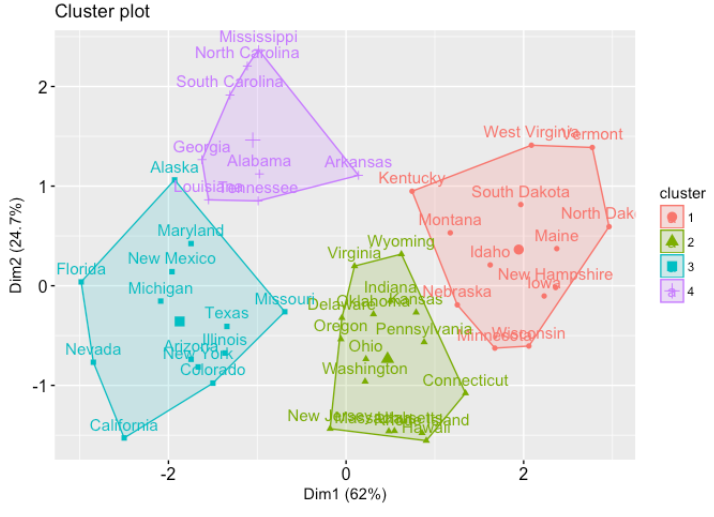
\includegraphics[width=0.6\textwidth]{../img/cluster-1.png}
    \caption{Ejemplo de clustering\cite{img-cluster-1}.}
\end{figure}

En la mayoría de las aplicaciones del AC se busca una partición de los datos en la que cada individuo u objeto pertenezca a un único cluster y el conjunto completo de clusters
contenga a todos los individuos. Sin embargo, esto no siempre es así y, de hecho, en algunas circunstancias, la superposición de clusters puede ofrecer una solución más aceptable.
Decimos que una respuesta aceptable del análisis cluster es que no se justifica la agrupación de los datos. El análisis cluster es un procedimiento objetivo; no están predefinidos,
sino que se forman a medida que avanza el análisis. \newline

Los datos básicos para la mayoría de las aplicaciones del análisis cluster se almacenan en una matriz $n \times p$, $X$, que contiene los valores de las variables que describen
cada objeto que se va a agrupar, es decir,

\[
X = [x_{ij}]_{i=1,\dots,n,\, j=1,\dots,p} =
\begin{bmatrix}
x_{11} & x_{12} & \cdots & x_{1p} \\
x_{21} & x_{22} & \cdots & x_{2p} \\
\vdots & \vdots & \ddots & \vdots \\
x_{n1} & x_{n2} & \cdots & x_{np}
\end{bmatrix}
\]
%       OBSERVA QUE ES LO CONTRARIO DE LO QUE DIJIMOS EN DATOS ÓMICOS (LA TRASPUESTA)?????? QUÉ HAGO?
donde $x_{ij}$ cuantifica la variable $j$ en la muestra $i$. El AC tratará de desarrollar un esquema de clasificación que particionará las filas de $X$ en $k$ clusters\cite{clustering-2}. %referencia: clustering-2.pdf


% medidas de proximidad (simularidad, disimilaridad)
\subsection{Medidas de proximidad}

Para desarrollar esta sección se han utlizado las siguientes referencias bibliográficas:\cite{Bib-5}\cite{clustering-2}. \newline%clustering-2 %Bib-5 \newline

Dado que el análisis cluster trata de identificar los vectores que son similares y agruparlos en clusters, es esencial contar con herramientas que permitan evaluar la cercanía o 
distancia entre los objetos que se están agrupando: las \textit{medidas de proximidad}. Las decisiones sobre cómo se van a formar los clusters dependen directamente de las medidas de proximidad utilizadas, ya que estas 
definen cómo se calcula la similitud o diferencia entre los distintos elementos. \newline

Si una medida de proximidad representa \textit{similaridad}, el valor de la medida incrementa 
cuanto más similares sean dos objetos. Alternativamente, si la medida de proximidad representa \textit{disimilitud}, el valor de la medida disminuye a medida que dos objetos se vuelven más 
parecidos.

\subsubsection{Medidas de Disimilaridad}

Cuando todas las variables registradas son continuas, las proximidades entre los individuos generalmente se cuantifican mediante medidas de disimilaridad o medidas de distancia. 
Por ello, definiremos el concepto de \textit{disimilaridad} análogamente al de distancia.

\begin{definicion}
    Sean $\Omega \subset \mathbb{R}^{n}$ un conjunto de puntos de $\mathbb{R}^{n}$ y $x,y \in \Omega$ dos puntos cualesquiera de dicho conjunto. Entendemos por disimilaridad a toda 
    aplicación $d: \Omega \times \Omega \longrightarrow \mathbb{R}$ que satisface las siguientes propiedades:

    \begin{itemize}
        \item[i)] $d(x,y) \ge 0$
        \item[ii)] $d(x,y)= 0 \Longleftrightarrow x = y$
        \item[iii)] $d(x,y) = d(y,x)$ (simétrica)
    \end{itemize}
    Se dice que la disimilaridad es \textit{métrica} si satisface una cuarta propiedad:
    \begin{itemize}
        \item[iv)] $d(x,y) \leq d(x,z) + d(z,y) \forall z \in \Omega$, 
    \end{itemize}
        
    y se dirá \textit{ultramétrica} si es métrica y además cumple:
        
    \begin{itemize}
        \item[v)] $d(x,y) \leq \max\{d(x,z),d(y,z)\}$
    \end{itemize}
        
\end{definicion}


A continuación presentamos algunas de las medidas de disimilaridad más usadas. Hemos de hacer notar que estas medidas normalmente se usan para medir cuán próximos están los individuos, 
pero si se quiere medir entre variables, también son válidas. Simplemente habría que trasponer la matriz $X$ y trabajar con ella. \newline

Toda la información que sigue a partir de este punto, ha sido extraída de las fuentes bibliográficas:\cite{Bib-1},\cite{Bib-5},\cite{Bib-6},\cite{clustering-2},\cite{clustering-1}.

% ejemplos para datos de intervalo, datos binarios ,etc.
\subsubsection{Medidas de disimilaridad}   % clustering-1, clustering-2, Bib-1, Bib-6, Bib-5

Las medidas de disimilaridad se usan ante la necesidad de agrupar objetos con características similares. Una medida de disimilaridad adecuada es la distancia entre 
dos observaciones. Se considera una medida de disimilaridad por el hecho de que la distancia aumenta conforme dos individuos se alejan. \newline

Una gran variedad de distancias pueden generarse mediante la norma\footnote[10]{Norma: Una \textit{norma} en un espacio vectorial $X$ es una aplicación $\|\cdot\| \rightarrow \mathbb{R}$ que verifica:
\begin{itemize}
    \item[(N.1)] Desigualdad triangular: $\|x+y\| \leq \|x\| + \|y\| \forall x,y \in X$
    \item[(N.2)] Homogeneidad por homotecias: $\|\lambda x\| = |\lambda| \|x\| \forall x \in \mathbb{X}$, $\lambda \in \mathbb{R}$
    \item[(N.3)] No degeneración: $x \in X$, $\|x\| = 0 \Rightarrow x = 0$.\cite{def-norma}  
\end{itemize}.} $L_{r}$, $r \geq 1$, 

% definición norma: https://www.ugr.es/~rpaya/documentos/AnalisisI/2014-15/Normados.pdf

\[
d_{ij} = \|x_{i} - x_{j}\|_{r} = \{\sum_{k=1}^{p} |x_{ik}-x_{jk}|^{r}\}^{\frac{1}{r}} \hspace{2cm} (1)
\]

donde $x_{ik}$ denota el valor de la $k$-ésima variable en el objeto $i$. A esta distancia se la conoce por el nombre de \textit{distancia de Minkowsi}\newline

En lo que sigue, consideremos $x_{i}, x_{j} \in \mathbb{R}^{p}$ dos individuos de la población. Esto es, dos filas de la matriz $X$ que contine los datos. 
Definimos las siguientes medidas de disimilaridad:

\begin{definicion}

Definimos la \textit{distancia euclídea} como la derivada de la norma $L_{2}$ (caso particular de la distancia de Minkowski cuando $r=2$), 

\[
d_{2}(x_{i},x_{j}) = \|x_{i} - x_{j}\|_{2} = \sqrt{(x_{i}-x_{j})^{'}(x_{i}-x_{j})} = \sqrt{\sum_{j=1}^{p}(x_{j}-y_{j})^{2}}
\] 

\end{definicion}


De entre todas las medidas de disimilaridad, y de todas las métricas de Minkowski, la distancia Euclidea es la más común. Hemos de tener en cuenta que la 
distancia euclidea (y la euclidea al cuadrado) suelen calcularse a partir de datos en bruto, 
no de datos estandarizados. Esto presenta varias ventajas (p. ej., la distancia entre dos objetos cualesquiera no se ve afectada por la adición de nuevos objetos 
al análisis, que podrían ser valores atípicos). Sin embargo, las distancias pueden verse considerablemente afectadas por las diferencias de escala entre las 
dimensiones a partir de las cuales se calculan.  Por ejemplo, si una de las dimensiones representa una longitud medida en centímetros y luego se convierte a milímetros (multiplicando los 
valores por 10), las distancias euclidianas o euclidianas al cuadrado resultantes (calculadas a partir de múltiples dimensiones) pueden verse considerablemente 
afectadas y, en consecuencia, los resultados de los análisis de conglomerados pueden ser muy diferentes. \newline


\begin{observacion}
La \textit{distancia euclidea al cuadrado} puede resultar útil para asignar progresivamente mayor importancia a los objetos más separados. Además, al evitar las
raíces cuadradas, los cálculos se amenizan.
\end{observacion}


\begin{definicion}

    Se denomina distancia \textit{Manhattan}, \textit{City Block}, \textit{Hamming}, o \textit{$d_{1}$}, a la distancia derivada de la norma $L_{1}$, que viene dada por
    
    \[
    d_{1}(x_{i},x_{j}) = \sum_{k=1}^{p} |x_{ik}-x_{jk}|
    \]
    
\end{definicion}

Se utiliza cuando todas las características (variables) son binarias y mide el número de características en las que dos individuos difieren.

\begin{definicion}  % referencia: https://en.wikipedia.org/wiki/Lp_space
    
    Tomando límite cuando $r \rightarrow \infty$, la distancia derivada del límite de la norma $L_{r}$, llamada \textit{norma del máximo}, $L_{\infty}$, es la que se conoce
    como \textit{distancia de Chebychev}, y viene dada por

    \[
    d_{\infty}(x_{i},x_{j}) = \max_{k=1,\dots,p} |x_{ik}-x_{jk}|
    \]
\end{definicion}

\begin{observacion}
    La distancia euclidea la podemos ver como un caso particular de la distancia:
    \[
    d_{M}(x_{i},x_{j}) = \sqrt{(x_{i}-x_{j})^{'}M(x_{i}-x_{j})}
    \]

    cuando $M=I_{p}$, la matriz identidad de orden $p$.
\end{observacion}

Supongamos que $M$ es la matriz de covarianzas de las variables (las columnas de la matrix $X$ de datos), que se define de la siguiente forma:

\[
M=\Sigma = \frac{1}{p} \sum_{i=1}^{n}(x_{ij}-\overline{x}_{j})(x_{ij}-\overline{x}_{j})^{'}, \hspace{0.2cm} j=1,...,p 
\]

Podemos observar que si $p \geq n$, la matriz de covarianzas $\Sigma$, es definida positiva y, por consiguiente, es invertible. Esto nos permite 
definir la siguiente medida de disimilaridad:

\begin{definicion}
    Definimos la \textit{distancia de Mahalanobis} para individuos, como:
    \[
    D_{\Sigma}(x_{i},x_{j}) = \sqrt{(x_{i}-x_{j})^{'}\Sigma^{-1}(x_{i}-x_{j})}
    \]
\end{definicion}

A diferencia de la distancia Euclidea, la de Mahalanobis es invariante frente a cambios de escala. En efecto, sea $C_{n\times n}$ una matriz no singular
de orden $n$, entonces:

\[
D_{\Sigma}(Cx_{i},Cx_{j}) = \sqrt{(Cx_{i},Cx_{j})^{'}[\frac{1}{p}C(x_{ij}-\overline{x}_{j})(x_{ij}-\overline{x}_{j})^{'}C^{'}]^{-1}(Cx_{i},Cx_{j})} = 
\]
\[
= \sqrt{(x_{i},x_{j})^{'}C^{'}(C^{'})^{-1}[\frac{1}{p}(x_{ij}-\overline{x}_{j})(x_{ij}-\overline{x}_{j})^{'}]^{-1}C^{-1}C(x_{i},x_{j})} = 
\]    
\[
= \sqrt{(x_{i}-x_{j})^{'}\Sigma^{-1}(x_{i}-x_{j})} = D_{\Sigma}(x_{i},x_{j})
\]

La distancia de Mahalanobis no se usa comúnmente en técnicas de clustering porque calcula la matriz $\Sigma$ considerando todos los individuos juntos, en lugar 
de tratar los objetos de cada clúster por separado. Además, su cálculo es más complejo que el de otras métricas. Sin embargo, puede aplicarse dentro de 
cada clúster en una fase específica del proceso\cite{cluster-mahalanobis}.


\subsection{Medidas de similaridad}

Esta subsección ha sido escrita en base a la información recogida en la referecia bibliográfica\cite{Bib-5}.

Como en la subsección anterior, consideremos $x_{i},x_{j}$ dos vectores cualesquiera de $\mathbb{R}^{p}$. \newline

\begin{definicion}
Sea $\Omega \subset{\mathbb{R}^{n}}$ un conjunto de puntos de $\mathbb{R^{p}}$. Llamaremos \textit{similaridad} a toda aplicación $s:\Omega \times \Omega \rightarrow \mathbb{R}$
que satisfaga las siguiente propiedades:

\begin{itemize}
    \item[i)] $0 \leq s(x_{i},x_{j}) \leq 1$
    \item[ii)]$s(x_{i},x_{j}) = 1$ si y solo si $x_{i} = x_{j}$
    \item[iii)] $s(x_{i},x_{j}) = s(x_{j},x_{i})$ (simétrica)
\end{itemize}
\end{definicion}

Las condiciones $(i)$ y $(ii)$ aseguran que toda similaridad es siempre positiva e identicamente $1$ cuando los objetos $i$ y $j$ sean iguales. \newline

\begin{observacion}
    Podemos formar una disimilaridad a partir de una similaridad, sin más que hacer:
    \[
    d_{ij} = 1 - s_{ij}
    \]
    u otra función decreciente. Sin embargo, a diferencia de las disimilaridades, no consituye una métrica. \newline
    Naturalmente, podríamos pensar si esto también ocurre a la inversa, es decir, si dada una medida de disimilaridad $d_{ij}$, podemos construir una medida de similaridad, sin más que 
    despejar $s_{ij}$ en la anterior expresión: 
    \[
    s_{ij} = 1/(1+d_{ij})
    \]
    Pero como $d_{ij}$ no está acotada superiormente, $s_{ij} \in (0,1]$, lo cual implica que $s_{ij} \neq 0$. Es por ello que no se pueden crear similaridades a partir de
    disimilaridades.
\end{observacion}

A continuación presentamos las principales medidas de similaridad que se usan en el ámbito del análisis cluster. \newline

\begin{definicion}
Definimos el \textit{coeficiente de correlación de Pearson} entre los objetos $x_{i},x_{j}$, como
\[
q_{ij} = \frac{\sum_{k=1}^{p}(x_{ik}-\overline{x}_{i.})(x_{jk}-\overline{x}_{j.})}{\left[\sum_{k=1}^{p}(x_{ik}-\overline{x}_{i.})^{2}\sum_{k=1}^{p}(x_{jk}-\overline{x}_{j.})^{2} \right]}
\]   
\end{definicion}

donde $\overline{x}_{i.} = \sum_{k=1}^{p}\frac{x_{ik}}{p}$ y $\overline{x}_{j.} = \sum_{k=1}^{p}\frac{x_{jk}}{p}$. \newline

\begin{observacion}
    Dado que $q_{ij} \in [-1,1]$, es claro que no satisface la primera condición necesaria para ser una similaridad. No obstante, esto cambia si consideramos en su lugar, el 
    valor absoluto del mismo, $|q_{ij}|$, o bien tomando $1-q_{ij}^{2}$. 
\end{observacion}

Presentamos ahora otra medida de similaridad para las filas de $X$.

\begin{definicion}
    Definimos el \textit{coseno del ángulo $\theta$} entre los vectores $x_{i},x_{j}$ como
    \[
    cos \theta = c_{ij} = \frac{x_{i}^{'}x_{j}}{\|x_{i}\| \|x_{j}\|}
    \]
\end{definicion}

\begin{observacion}
    Podemos ver que estamos en la misma situación que antes, $c_{ij} \in [-1,1]$, lo cual indica que no verifica la propiedad $1$ de las medidas de similaridad. La solución a esto es 
    la misma que en el caso anterior: trabajar con $\|q_{ij}\|$ o $\|1-q_{ij}^{2}\|$. \newline
\end{observacion}

% clústering jerárquico

\subsection{Métodos jerárquicos}  % Bib-1, Bib-2, Bib-5, bejar-AC-2, gallardo-jerarquicos

Los \textit{métodos jerárquicos} para el análisis cluster representan un intento de encontrar buenos clusters en los datos mediante la combinación o división de clusters, con el prósito de
minimizar (maximizar) una medida de disimilaridad (similaridad). Hay dos tipos de métodos jerárquicos: los \textit{aglomerativos} y los \textit{disociativos}. Los aglomerativos comienzan 
con clusters que contienen un solo objeto y sucesivamente van combinando clusters hasta que todos forman un único cluster. Los disociativos, por su parte, hacen justo lo contrario: 
comienzan con todos los objetos agrupados en un único cluster, a continuación dividen dicho cluster en dos clusters separados, y así sucesivamente hasta formar clusters con un solo objeto. 

\begin{observacion}
Aunque se le suele prestar más atención a los métodos aglomerativos, los disociativos proporcionan clusterings más sofisticados y robustos.
\end{observacion}

\subsubsection{Dendrograma}

El resultado final de todo método jerárquico es lo que se conoce como \textit{dendograma} o \textit{diagrama en árbol jerárquico}. Es una representación gráfica del clústering que generalmente se
dibuja en sentido inverso, comenzando desde el último cluster que se ha formado y que engloba a todos los objetos y desde similaridad 0. En el punto de similaridad donde dos clusters se combinan 
para dar lugar al cluster final, este se divide en dos clusters padres y así sucesivamente; la solución con $k$ clusters se obtiene fusionando algunos clusters de la solución con $(k+1)$. \newline

El dendrograma puede dibujarse horizontal o verticalmente, queda a elección de cada uno; ambas formas proporcionan la misma información. En nuestro caso, lo consideraremos en vertical. Nos permite 
determinar la altura del criterio de unión a la que los clusters se combinan para formar un nuevo cluster más grande. Los elementos similares se combinan a alturas bajas, mientras que los elementos
más disímiles se combinan a mayor altura en el dendrograma. Por lo tanto, es la diferencia de alturas la que define la proximidad de los individuos entre sí. Cuanto mayor sea la distancia entre las
alturas a las que se combinan los clusters, más fácilmente podremos identificar la estructura sustancial de los datos. \newline

Cortando el dendrograma a una altura adecuada, podremos obtener una partición de los datos en un número específico de grupos. Si dibujamos una línea horizontal a una altura adecuada, el número, $k$, de 
líneas verticales intersecadas por dicha línea horizontal determina una solución con $k$ clusters. Por tanto, estamos diciendo que cada intersección de la horizontal con una de las $k$ líneas verticales
representa un cluster y los elementos que están por debajo de dicha intersección serán los elementos que conforman el cluster. \newline

Nos podemos preguntar cómo saber a qué altura cortar el dendrograma. La respuesta es que depende; deberemos cortar a aquella altura que mejor represente los datos de entrada.\newline % bejar-AC-2

\begin{nota}
    
    Cabe remarcar que, si bien las distancias verticales son importantes a la hora de determinar una solución, las horizontales son totalmente irrelevantes. \newline

\end{nota}

\begin{ejemplo}

    Vemos qué información nos puede dar este dendrograma sobre el número de clusters, aproximado, en los que podríamos agrupar un conjunto de datos:

    \begin{figure}[h]
        \centering
        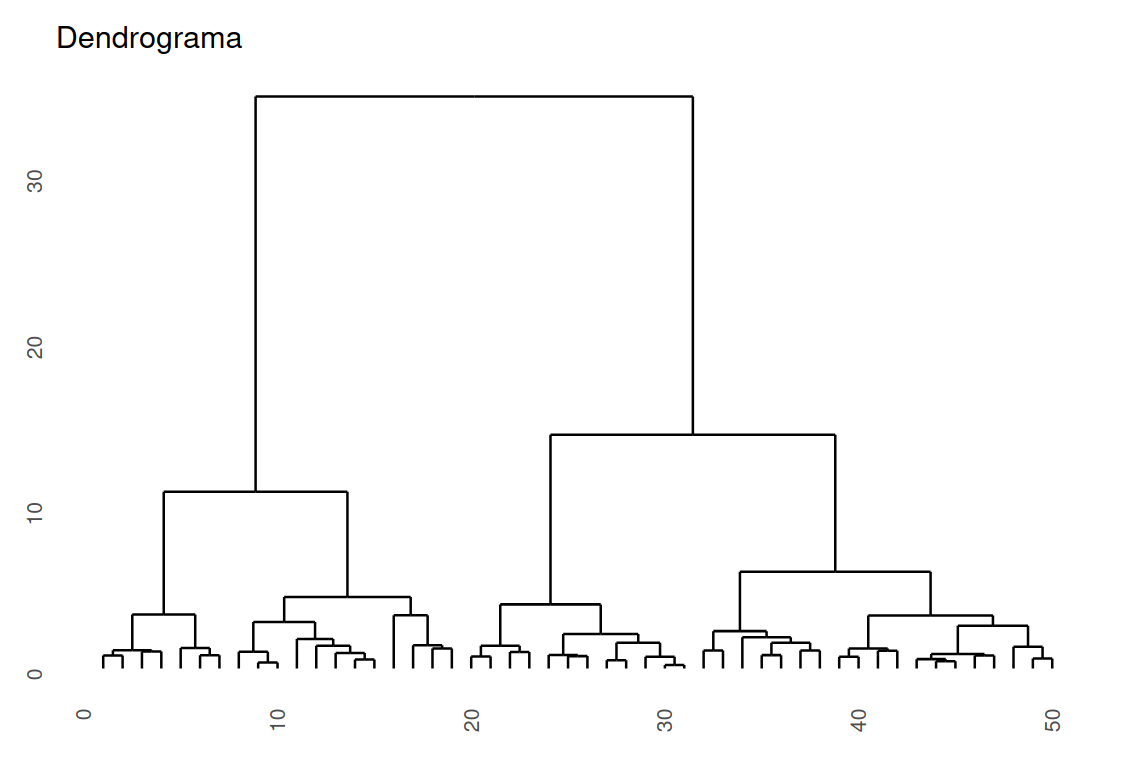
\includegraphics[width=0.5\textwidth]{../img/dendrograma-1.png}
        \caption{Ejemplo de dendrograma.}
    \end{figure}

    \FloatBarrier

    Aclaremos que en el eje vertical tenemos la \textit{distancia euclidea} que existe entre cada grupo y en el eje horizontal, los datos. Las línea verticales son los
    agrupamientos que, a medida que vamos subiendo, van disminuyendo, hasta acabar en uno solo. Observamos que hay una gran separación entre las ramas en un entorno alrededor
    de $10$, por lo que, si trazáramos una línea horizontal a una altura por encima o por debajo de $10$, identificamos $3$ y $4$ clusters, respectivamente. \newline

    No podemos afirmar nada acerca del número de clusters óptimo con esta información. Habría que utilizar otros métodos, tanto visuales como matemáticos que nos permitan
    hacer una afirmación acerca de $k$ un poco más rotunda.

\end{ejemplo}


\subsubsection{Métodos jerárquicos aglomerativos}  %gallardo y Bib-5

En esta subsección vamos a analizar los principales métodos jerárquicos aglomerativos. Hemos de aclarar que ninguno de los que presentaremos es más eficiente que otro. Esto 
dependerá de la naturaleza de los datos y el enfoque que tenga el análisis. \newline

\textbf{Estrategia de la distanca mínima o máxima similaridad} \newline

Del inglés \textit{single linkage}, traducido como \textit{encadenamiento simple}, y más conocida como la estrategia del \textit{vecino más cercano} es una estrategia que
se basa en combinar dos clusters que tengan distancia mínima (o máxima similaridad), siendo esta la distancia mínima entre sus componentes. \newline

Sean $C_{i}$ y $C_{j}$ dos clusters cualesquiera con $n_{i}$, $n_{j}$ elementos, respectivamente, y sean $x^{i}_{k} \in C_{i}$ , $x^{j}_{m} \in C_{j}$, con $k=1,\dots,n_{i}$, $m=1,\dots,n_{j}$ dos elementos de dichos clusters. La 
distancia entre $C_{i}$ y $C_{j}$ viene dada por

\[
d(C_{i},C_{j}) = \min_{\substack{k=1,\dots,n_{i} \\ m=1,\dots,n_{j}}}\{d(x^{i}_{k},x^{j}_{m}) \text{ | } x^{i}_{k} \in C_{i} \text{ y } x^{j}_{m} \in C_{j}\}
\]

donde $d(x^{i}_{k},x^{j}_{m})$ es la distancia Euclidea, generalmente, o cualquier otra distancia entre los elementos $x^{i}_{k},x^{j}_{k}$ de los clusters. 

Equivalentemente, en un contexto en el que usemos similaridad, se unirán dos clusters $C_{i}, C_{j}$ si

\[
s(C_{i},C_{j}) = \max_{\substack{k=1,\dots,n_{i} \\ m=1,\dots,n_{j}}}\{s(x^{i}_{k},x^{j}_{m}) \text{ | } x^{i}_{k} \in C_{i} \text{ y } x^{j}_{m} \in C_{j}\}
\]

\textbf{Estrategia de la distancia máxima o mínima similaridad}

Conocido también como el método del encadenamiento completo, al contrario que en la estrategia anterior, esta se basa en calcular la distancia máxima 
entre los clusters teniendo en cuenta la distancia máxima entre sus componentes. Esto es, ponemos el foco de atención en los elementos más dispares de 
los clusters, es decir, los que están a mayor distancia o son menos símiles. \newline

Sean entonces $C_{i}$ y $C_{j}$ dos clusters cualesquiera con $n_{i}$, $n_{j}$ elementos, respectivamente y sean $x^{i}_{k} \in C_{i}$ , $x^{j}_{m} \in C_{j}$, 
con $k=1,\dots,n_{i}$, $m=1,\dots,n_{j}$ dos elementos de dichos clusters. Entonces, la distancia entre dichos clusters viene dada por:

\[
d(C_{i},C_{j}) = \max_{\substack{k=1,\dots,n_{i} \\ m=1,\dots,n_{j}}}\{d(x^{i}_{k},x^{j}_{m}) \text{ | } x^{i}_{k} \in C_{i} \text{ y } x^{j}_{m} \in C_{j}\}
\]

Equivalentemente, si lo miramos desde el punto de vista de la similaridad, se unirán dos clusters $C_{i}, C_{j}$ si

\[
s(C_{i},C_{j}) = \min_{\substack{k=1,\dots,n_{i} \\ m=1,\dots,n_{j}}}\{s(x^{i}_{k},x^{j}_{m}) \text{ | } x^{i}_{k} \in C_{i} \text{ y } x^{j}_{m} \in C_{j}\}
\]

\textbf{Estrategia de la distancia o similitud promedio}

Mientras que en las dos estrategias anteriores la combinación de dos clusters en uno dependía únicamente de un único para de objetos dentro de cada cluster, 
y se usaba la distancia máxima o mínima, la estrategia de la distancia promedio calcula la distancia entre dos clusters como el promedio de las disimilaridades 
en cada cluster. Dependiendo de si consideramos el tamaño de los clusters en el promedio o no, podemos distinguir entre dos estrategias diferentes: la no ponderada
y la ponderada. \newline

Consideremos en lo que sigue dos clusters $C_{i}$, $C_{j}$ con $n_{i},n_{j}$ elementos, y $x^{i}_{k},x^{j}_{m}$ dos elementos de $C_{i},C_{j}$, respectivamente con $k=1,\dots,n_{i}$, $m=1,\dots,n_{j}$.

\begin{itemize}
    \item \textbf{No ponderada} \newline

    Supongamos, sin pérdida de generalidad, que $C_{i}$ está constituido por dos clusters $C_{i_{1}}$ y $C_{i_{2}}$ con $n_{i_{1}},n_{i_{2}}$ elementos respectivamente, la distancia entre $C_{i}$ y $C_{j}$ viene dada por
    \[
    d(C_{i},C_{j}) = \frac{d(C_{i_{1}}, C_{j}) + d(C_{i_{2}}, C_{j})}{2}
    \]

    Observamos que esta distancia es independiente de los tamaños de los clusters involucrados. Esto quiere decir que las distancias respecto a $C_{j}$ de $C_{i_{1}}$ y $C_{i_{2}}$
    tienen el mismo peso. 

    \item \textbf{Ponderada} \newline
    
    A diferencia de la anterior estrategia, esta distancia es el promedio ponderado de las distancias de las componentes del cluster con respecto a las del otro. Supongamos que 
    $C_{i}$ está constituido por dos clusters $C_{i_{1}}$, $C_{i_{2}}$ con $n_{i_{1}}$,$n_{i_{2}}$ elementos tales que $n_{i} = n_{i_{1}}+n_{i_{2}}$ y tomemos los elementos $x^{i_{1}}_{z} \in C_{i_{1}}$, $x^{i_{2}}_{w} \in C_{i_{2}}$, donde 
    $z = 1,\dots,n_{i_{1}} $ y $w = 1,\dots,n_{i_{2}}$. Entonces, la distancia promedio pondera entre $C_{i},C_{j}$ viene dada por
    
    \[
    d(C_{i},C_{j}) = \frac{\sum_{k=1}^{n_{i}}\sum_{m=1}^{n_{j}}d(x^{i}_{k},x^{j}_{m})}{n_{i}n_{j}} = \frac{1}{(n_{i_{1}}+n_{i_{2}})n_{j}} \sum_{k=1}^{n_{i_{1}}+n_{i_{2}}} \sum_{m=1}^{n_{j}} d(x^{i}_{k},x^{j}_{m}) = 
    \]
    \[
    = \frac{1}{(n_{i_{1}}+n_{i_{2}})n_{j}} \sum_{z=1}^{n_{i_{1}}} \sum_{m=1}^{n_{j}} d(x^{i_{1}}_{z},x^{j}_{m}) + \frac{1}{(n_{i_{1}}+n_{i_{2}})n_{j}} \sum_{w=1}^{n_{i_{2}}} \sum_{m=1}^{n_{j}} d(x^{i_{2}}_{w},x^{j}_{m}) = 
    \]
    \[
    = \frac{n_{i_{1}}}{(n_{i_{1}}+n_{i_{2}})n_{j}n_{i_{1}}} \sum_{z=1}^{n_{i_{1}}} \sum_{m=1}^{n_{j}} d(x^{i_{1}}_{z},x^{j}_{m}) + \frac{n_{i_{2}}}{(n_{i_{1}}+n_{i_{2}})n_{j}n_{i_{2}}} \sum_{w=1}^{n_{i_{2}}} \sum_{m=1}^{n_{j}} d(x^{i_{2}}_{w},x^{j}_{m}) = 
    \]
    \[
    = \frac{n_{i_{1}}}{n_{i_{1}}+n_{i_{2}}} d(C_{i_{1}},C_{j}) + \frac{n_{i_{2}}}{n_{i_{1}}+n_{i_{2}}} d(C_{i_{2}},C_{j}) = 
    \]
    \[
    = \frac{n_{i_{1}}d(C_{i_{1}},j) + n_{i_{2}}d(C_{i_{2}},C_{j})}{n_{i_{1}}+n_{i_{2}}}
    \]

\end{itemize}

\vspace{0.5cm}

\textbf{Método del centroide} \newline  % gallardo y Bib-5

En este método, para determinar cuán semejantes son dos clusters, vamos a poner el foco de atención en los \textit{centroides} de los mismos, es decir, en los vectores de medias de las variables 
observadas sobre los individuos que conforman el cluster. Entonces, los centroides de los clusters $C_{i},C_{j}$ son

\[
\bar{x}^{i} = \frac{\sum_{k=1}^{n_{i}}x^{i}_{k}}{n_{i}} = \begin{bmatrix} \bar{x}^{i}_{1} \\  \bar{x}^{i}_{2} \\ \vdots \\ \bar{x}^{i}_{n_{i}} \end{bmatrix} \text{ y } \bar{x}^{j} = \frac{\sum_{m=1}^{n_{j}}x^{j}_{m}}{n_{j}} = \begin{bmatrix} \bar{x}^{j}_{1} \\  \bar{x}^{j}_{2} \\ \vdots \\ \bar{x}^{j}_{n_{j}} \end{bmatrix} 
\]

respectivamente, y el cuadrado de la distancia Euclidea entre ambos centroides es $d^{2}(C_{i},C_{j}) = \|\bar{x}^{i} - \bar{x}^{j}\|^{2}$. Se persigue entonces el objetivo de encontrar clusters que hagan mínima la 
distancia entre sus centroides, para, consecuentemente, combinarlos en un nuevo cluster, que llamaremos $C_{t}$ con centroide $\bar{x}^{t} = \frac{(n_{i}\bar{x}^{i} + n_{j}\bar{x}^{j})}{n_{i}+n_{j}}$. Se calcularían 
de nuevo las distancias entre dicho centroide y el de los demás clusters. Continuaríamos el proceso hasta obtener un único cluster.\newline

El método del centroide se denomina \textit{método de la mediana} si se utiliza un promedio no ponderado de los centroides: $\bar{x}^{t} = \frac{(\bar{x}^{i} +\bar{x}^{j})}{2}$. Este método es preferible cuando $n_{i} >> n_{j}$ o
viceversa. \newline

Calculamos el cuadrado de la distancia Euclidea entre el cluster $C_{t}$ y el centroide $\bar{x}^{u}$ de un tercer cluster $C_{u}$ de la siguiente forma:
\[
d^{2}(C_{t}, C_{u}) = \left( \frac{n_{i}}{n_{i} + n_{j}} \right) d^{2}(C_{i},C_{j}) + \left (\frac{n_{j}}{n_{i} + n_{j}}\right) d^{2}(C_{i},C_{u}) - \left( \frac{n_{i}n_{j}}{n_{i} + n_{j}}\right) d^{2}(C_{i},C_{j})
\]

\vspace{0.5cm}

\textbf{Método de Ward} \newline

El \textit{método de Ward}, también conocido como \textit{método de la suma incremental de cuadrados}, es un método jerárquico aglomerativo cuya filosofía la podemos resumir de la siguiente forma: \newline

Supongamos que tenemos $m$ elementos que queremos agrupar. Comenzamos con $m$ clusters, cada uno de ellos con un único individuo. A continuación, estudiamos la similaridad de dichos clusters y, el par de clusters más
similares se combinan, reduciendose el número de clusters en uno. Se sigue este proceso hasta que todos los clusters estén fusionados. El objetivo de este método es, en definitiva, encontrar en cada iteración, los dos 
clusters tales que su fusión genere el menor incremento en el valor total de la suma de los cuadrados de las diferencias entre cada elemento y el centroide del cluster. \newline

Para desarrollar formalmente el método, vamos a establecer la siguiente notación:

\begin{itemize}
    \item Notaremos por $x^{k}_{ij}$ al valor de la $j$-ésima variable observada sobre el $i$-ésimo individuo dentro del $k$-ésimo cluster. Suponemos que dicho cluster estará formado por $n_{k}$ indivduos.
    \item Al centroide del $k$-ésimo cluster lo denotaremos como hicimos en el método del centroide: $m^{k}$, con $n$ componentes, $m^{k}_{j}$.
    \item $E_{k}$ será la suma de los cuadrados de las distancias (distancia euclidea) de cada individuo del cluster $k$ al centroide (los errores del cluster $k$). Esto es,
    \[
    E_{k} = \sum_{i=1}^{n_{k}}\sum_{j=1}^{n}(x^{k}_{ij} - m^{k}_{j})^{2} = \sum_{i=1}^{n_{k}}\sum_{j=1}^{n}(x^{k}_{ij})^{2} - n_{k}\sum_{j=1}^{n}(m^{k}_{j})^{2}
    \]
    \item Llamaremos $E$ a la suma de los cuadrados de los errores de todos los clusters en su conjunto. Es decir, suponiendo que hubiera $h$ clusters
    \[
    E = \sum_{k=1}^{h} E_{k}
    \]
\end{itemize}


\begin{observacion}
    Notemos que al principio del método, $E_{k} = 0$, $\forall k \in \{1,\dots,m\}$ pues hay $m$ clusters compuestos por un solo individuo. \newline
    En cada etapa, buscaremos los dos clusters cuya fusión minimce el incremento en $E$.
\end{observacion}

Supongamos que en la siguiente etapa son $C_{p}$ y $C_{q}$ los dos clusters que se fusionan en uno nuevo, $C_{t}$. Entonces, el incremento de $E$, $\Delta E_{pq}$, vendrá dado por
\[
\Delta E_{pq} = E_{t} - E_{p} - E_{q} =
\]
\[
= \left[ \sum_{i=1}^{n_{t}}\sum_{j=1}^{n}(x^{t}_{ij})^{2} - n_{t}\sum_{j=1}^{n}(m^{p})^{2} \right] - \left[ \sum_{i=1}^{n_{k}}\sum_{j=1}^{n}(x^{p}_{ij})^{2} - n_{p}\sum_{j=1}^{n}(m^{p})^{2} \right] - \left[ \sum_{i=1}^{n_{q}}\sum_{j=1}^{n}(x^{q}_{ij})^{2} - n_{p}\sum_{j=1}^{n}(m^{q})^{2} \right] = 
\]
\[
\overset{n_{t} = n_{p}+n_{q}}{=} n_{p}\sum_{j=1}^{n}(m^{p}_{j})^{2} + n_{q}\sum_{j=1}^{n}(m^{q}_{j})^{2} - n_{t}\sum_{j=1}^{n}(m^{t}_{j})^{2}
\]

Ahora, por un lado sabemos por el apartado anterior que el centroide de un cluster $C_{c}$ se calcula como 
\[
m^{c} = \frac{\sum_{j=1}^{n_{c}}x^{c}_{j}}{n_{c}}
\]

Aplicando esto al cluster $C_{p}$, tenemos:
\[
m^{p} = \frac{\sum_{j=1}^{n_{p}}x^{p}_{j}}{n_{p}} \Longleftrightarrow n_{p}m^{p} = \sum_{j=1}^{n_{p}}x^{p}_{j}
\]

Para el cluster $C_{q}$:
\[
m^{q} = \frac{\sum_{j=1}^{n_{q}}x^{q}_{j}}{n_{q}} \Longleftrightarrow n_{q}m^{q} = \sum_{j=1}^{n_{q}}x^{q}_{j}
\]

Cuando fusionamos los clusters $C_{p}$ y $C_{q}$, tenemos un cluster $C_{t}$ de $n_{t} = n_{p} + n_{q}$ elementos, con centroide
\[
m^{t} = \frac{\sum_{j=1}^{n_{t}}x^{t}_{j}}{n_{t}}
\]

Como $C_{t}$ tiene todos los puntos de $C_{p}$ y $C_{q}$, podemos escribir
\[
\sum_{j=1}^{n_{t}}x^{t}_{j} = \sum_{j=1}^{n_{p}}x^{p}_{j} + \sum_{j=1}^{n_{q}}x^{q}_{j}
\]

Por lo que, si sustituimos en las expresiones de $n_{p}m^{p}$ y $n_{q}m^{q}_{j}$:
\[
\sum_{j=1}^{n_{t}}x^{t}_{j}  = n_{p}m^{p} + n_{q}m^{q}
\]

Multiplicando por $n_{t}$, obtenemos:
\[
n_{t}m^{t} = n_{p}m^{p} + n_{q}m^{q}
\]

Como esto es una igualdad vectorial, la igualdad se verifica componente a componente:

\[
n_{t}m^{t}_{j} = n_{p}m^{p}_{j} + n_{q}m^{q}_{j} \text{ con } j = 1,\dots,n
\]

Partiendo entonces de la igualdad $n_{t}m^{t}_{j} = n_{p}m^{p}_{j} + n_{q}m^{q}_{j}$, elevando al cuadrado ambos miembros obtenemos
\[
n_{t}^{2}(m^{t}_{j})^{2} = n^{2}_{p}(m^{p}_{j})^2 + n^{2}_{q}(m^{q}_{j})^{2} + 2n_{p}n_{q}m^{p}_{j}m^{q}_{j} = 
\]
\[
= n^{2}_{p}(m^{p}_{j})^2 + n^{2}_{q}(m^{q}_{j})^{2} + n_{p}n_{q}(2m_{j}^{p}m_{j}^{q}) = n^{2}_{p}(m^{p}_{j})^2 + n^{2}_{q}(m^{q}_{j})^{2} + n_{p}n_{q}((m_{j}^{p})^{2} + (m_{j}^{q})^{2} - (m^{p}_{j}-m^{q}_{j})^{2})
\]

de donde se obtiene
\[
n_{t}^{2}(m^{t}_{j})^{2} = n_{p}(n_{p}+n_{q})(m^{p}_{j})^{2} + n_{q}(n_{p}+n_{q})(m^{q}_{j})^{2} - n_{p}n_{q}(m_{j}^{p}-m_{j}^{q})^{2}
\]

Dividiendo por $n_{t}^{2}$ se obtiene
\[
(m_{j}^{t})^{2} = \frac{n_{p}}{n_{t}}(m^{p}_{j})^{2} + \frac{n_{q}}{n_{t}}(m_{j}^{q})^{2} - \frac{n_{p}n_{q}}{n_{t}^{2}}(m^{p}_{j}-m^{q}_{j})^{2}
\]

Por tanto, si sustituimos esta expresión en la del incremento, $\Delta E_{pq}$, nos queda lo siguiente:
\[
\Delta E_{pq} = n_{p}\sum_{j=1}^{n}(m^{p}_{j})^{2} + n_{q}\sum_{j=1}^{n}(m^{q}_{j})^{2} - n_{t}\sum_{j=1}^{n} \left[\frac{n_{p}}{n_{t}}(m^{p}_{j})^{2} + \frac{n_{q}}{n_{t}}(m_{j}^{q})^{2} - \frac{n_{p}n_{q}}{n_{t}^{2}}(m^{p}_{j}-m^{q}_{j})^{2}\right] \Longleftrightarrow
\]
\[
\Longleftrightarrow \Delta E_{pq} = n_{p}\sum_{j=1}^{n}(m^{p}_{j})^{2} + n_{q}\sum_{j=1}^{n}(m^{q}_{j})^{2} - m_{p}\sum_{j=1}^{n}(m_{j}^{p})^{2} - n_{q}\sum_{j=1}^{n}(m^{q}_{j})^{2} + \frac{n_{p}n_{q}}{n_{t}}\sum_{j=1}^{n}(m^{p}_{j}-m^{q}_{j})^{2}
\]
\vspace{0.5cm}
\[
\Rightarrow \Delta E_{pq} = \frac{n_{p}n_{q}}{n_{t}}\sum_{j=1}^{n}(m^{p}_{j}-m^{q}_{j})^{2}
\]

Obtenemos por consiguiente que el menor incremento de los errores cuadráticos es proporcional al cuadrado de la distancia euclidea de los centroides de los clusters fusionados. \newline

Veamos cómo calcular los incrementos a partir de otros ya previamente calculados. \newline
Sea $C_{t}$ el cluster que resulta de fusionar $C_{p}$ y $C_{q}$ y consideremos ahora otro cluster $C_{r}$ distinto a los demás. Entonces, por lo visto anteriormente, 
el incremento en $E$ que se produce al fusionar $C_{r}$ con $C_{t}$, viene dado por
\[
\Delta E_{rt} = \frac{n_{r}n_{t}}{n_{r}+n_{t}}\sum_{j=1}^{n}(m^{r}_{j}-m^{t}_{j})^{2}
\]

Como $n_{t}m^{t} = n_{p}m^{p} + n_{q}m^{q}$ y $n_{t} = n_{p}+n_{q}$, y sabemos también que $(m_{j}^{t})^{2} = \frac{n_{p}}{n_{t}}(m^{p}_{j})^{2} + \frac{n_{q}}{n_{t}}(m_{j}^{q})^{2} - \frac{n_{p}n_{q}}{n_{t}^{2}}(m^{p}_{j}-m^{q}_{j})^{2}$, deducimos que
\[
(m^{r}_{j}-m^{t}_{j})^{2} = (m^{r}_{j})^{2} + (m^{t}_{j})^{2} - 2m_{j}^{r}m_{j}^{t} = 
\]
\[
= (m_{j}^{r})^{2} + \frac{n_{p}}{n_{t}}(m^{p}_{j})^{2} + \frac{n_{q}}{n_{t}}(m^{q}_{j})^{2} - \frac{n_{p}n_{q}}{n_{t}^{2}}(m^{p}_{j}-m^{q}_{j})^{2} - 2m^{r}_{j}\frac{n_{p}m^{p}_{j} + n_{q}m^{q}_{j}}{n_{t}} = 
\]
\[
= \frac{n_{p}(m_{j}^{r})^{2}+n_{q}(m_{j}^{q})^{2}}{n_{t}} + \frac{n_{p}}{n_{t}}(m^{p}_{j})^{2} + \frac{n_{q}}{n_{t}}(m^{q}_{j})^{2} - \frac{n_{p}n_{q}}{n^{2}_{t}}(m^{p}_{j}-m^{q}_{j})^{2} - 2m^{r}_{j}\frac{n_{p}m^{p}_{j} + n_{q}m^{q}_{j}}{n_{t}} = 
\]
\[
= \frac{n_{p}}{n_{t}}(m^{r}_{j} - m^{p}_{j})^{2} + \frac{n_{q}}{n_{t}}(m^{r}_{j} - m^{q}_{j})^{2} - \frac{n_{p}n_{q}}{n_{t}^{2}}(m^{p}_{j}-m^{q}_{j})^{2}
\]

Obtenemos por tanto,

\[
\Delta E_{rt} = \frac{n_{r}n_{t}}{n_{r}+n_{t}} \sum_{j=1}^{n} (m^{r}_{j}-m^{t}_{j})^{2} = 
\]
\[
= \frac{n_{r}n_{t}}{n_{r}+n_{t}}\sum_{j=1}^{n} \left[\frac{n_{p}}{n_{t}}(m^{r}_{j} - m^{p}_{j})^{2} + \frac{n_{q}}{n_{t}}(m^{r}_{j} - m^{q}_{j})^{2} - \frac{n_{p}n_{q}}{n_{t}^{2}}(m^{p}_{j}-m^{q}_{j})^{2}\right] = 
\]
\[
= \frac{n_{r}n_{p}}{n_{r}+n_{t}}\sum_{j=1}^{n} (m^{r}_{j} - m^{p}_{j})^{2} + \frac{n_{q}n_{r}}{n_{r}+n_{t}}\sum_{j=1}^{n}(m^{r}_{j} - m^{q}_{j})^{2} - \frac{n_{r}n_{p}n_{q}}{n_{t}(n_{r}+n_{t})}(m^{p}_{j}-m^{q}_{j})^{2} = 
\]
\[
= \frac{1}{n_{r}+n_{t}}\sum_{j=1}^{n}\left[n_{r}n_{p}(m^{r}_{j}-m^{p}_{j})^{2} + n_{r}n_{q}(m^{r}_{j}-m^{q}_{j})^{2} - \frac{n_{r}n_{p}n_{q}}{n_{p}+n_{q}}(m^{p}_{j}-m^{q}_{j})^{2}\right] =
\]
\[
= \frac{1}{n_{r}+n_{t}}[(n_{r}+n_{p})\Delta E_{rp} + (n_{r}+n_{q})\Delta E_{rq} - n_{r}\Delta E_{pq}]
\]

\vspace{0.5cm}

\begin{nota}
    Se puede demostrar que esta relación no depende de la forma específica en que se mide la distancia, siempre que esta se defina a partir de 
    una norma inducida por un producto escalar o que satisfaga la ley del paralelogramo.
\end{nota}

\vspace{0.5cm}

Ofrecemos a continuación un pequeño ejemplo de aplicación de este método aglomerativo.

\begin{ejemplo}

    Consideremos los siguientes datos de $5$ genotipos sobre los que se observan dos variables $X_{1}$ y $X_{2}$.

    \begin{table}[h]
        \centering
        \begin{tabular}{|c|c|c|}
            \hline
            \textbf{Genotipo} & \textbf{$X_{1}$} & \textbf{$X_{2}$} \\
            \hline
            $G_{1}$ & 7 & 10 \\
            \hline
            $G_{2}$ & 8 & 10 \\
            \hline
            $G_{3}$ & 6 & 5 \\
            \hline
            $G_{4}$ & 3 & 2 \\
            \hline
            $G_{5}$ & 11 & 10 \\
            \hline
            
        \end{tabular}
        \caption{Ejemplo método de Ward}

    \end{table}
    
    En la primera iteración del método, contamos con $5$ clusters, cada uno compuesto por un único punto (cada punto de nuestro dataset 
    en un cluster):

    \begin{table}[h]
        \centering
        \begin{tabular}{|c|c|c|c|c|}
            \hline
            \textbf{Partición} & \textbf{Centroides} & \textbf{$E_{k}$} & \textbf{$E$} & \textbf{$\Delta E$} \\
            \hline
            $G_{1},G_{2},G_{3},G_{4},G_{5}$ & los propios puntos & $E_{G_{1}} = E_{G_{2}}=E_{G_{3}}=E_{G_{4}}=E_{G_{5}}=0$ & $0$ & $0$ \\
            \hline
        \end{tabular}
        \caption{Nivel 0} 

    \end{table}

    A continuación, barajamos todas las parejas que podemos formar con estos $5$ elementos, para estudiar qué pareja de clusters generaría el menor
    $\Delta E$ al fusionarse. Estudiemos entonces las $\binom{5}{2} = 10$ combinaciones posibles.

    \begin{table}[h]
        \small
        \centering
        \begin{tabular}{| c | c | c | c | c |}
            \hline
            \textbf{Partición} & \textbf{Centroides} & \(E_{k}\) & \(E\) & \(\Delta E\) \\
            \hline
            (\(G_{1}, G_{2}\)), \(G_{3}, G_{4}, G_{5}\) & \(C_{G_{1}G_{2}} = (7.5, 10)\) & \(E_{G_{1}G_{2}} = 0.5\) & 0.5 & 0.5 \\
            \hline
            (\(G_{1}, G_{3}\)), \(G_{2}, G_{4}, G_{5}\) & \(C_{G_{1}G_{3}} = (6.5, 7.5)\) & \(E_{G_{1}G_{3}} = 13\) & 13 & 13 \\
            \hline
            (\(G_{1}, G_{4}\)), \(G_{2}, G_{3}, G_{5}\) & \(C_{G_{1}G_{4}} = (5, 6)\) & \(E_{G_{1}G_{4}} = 40\) & 40 & 40 \\
            \hline
            (\(G_{1}, G_{5}\)), \(G_{2}, G_{3}, G_{4}\) & \(C_{G_{1}G_{5}} = (9, 10)\) & \(E_{G_{1}G_{5}} = 8\) & 8 & 8 \\
            \hline
            (\(G_{2}, G_{3}\)), \(G_{1}, G_{4}, G_{5}\) & \(C_{G_{2}G_{3}} = (7, 7.5)\) & \(E_{G_{2}G_{3}} = 14.5\) & 14.5 & 14.5 \\
            \hline
            (\(G_{2}, G_{4}\)), \(G_{1}, G_{3}, G_{5}\) & \(C_{G_{2}G_{4}} = (5.5, 6)\) & \(E_{G_{2}G_{4}} = 44.5\) & 44.5 & 44.5 \\
            \hline
            (\(G_{2}, G_{5}\)), \(G_{1}, G_{3}, G_{4}\) & \(C_{G_{2}G_{5}} = (9.5, 10)\) & \(E_{G_{2}G_{5}} = 4.5\) & 4.5 & 4.5 \\
            \hline
            (\(G_{3}, G_{4}\)), \(G_{1}, G_{2}, G_{5}\) & \(C_{G_{3}G_{4}} = (4.5, 3.5)\) & \(E_{G_{3}G_{4}} = 9\) & 9 & 9 \\
            \hline
            (\(G_{3}, G_{5}\)), \(G_{1}, G_{2}, G_{4}\) & \(C_{G_{3}G_{5}} = (8.5, 7.5)\) & \(E_{G_{3}G_{5}} = 25\) & 25 & 25 \\
            \hline
            (\(G_{4}, G_{5}\)), \(G_{1}, G_{2}, G_{3}\) & \(C_{G_{4}G_{5}} = (7, 6)\) & \(E_{G_{4}G_{5}} = 64\) & 64 & 64 \\
            \hline
        \end{tabular}
        \caption{Nivel 1}
        
    \end{table}

    Observamos que se han de fusonar los elementos $G_{1}$ y $G_{2}$. En este nivel, la configuración de clusters es $(G_{1},G_{2}),G_{3},G_{4},G_{5}$. \newline

    A continuación, calculemos los incrementos que daría lugar las $\binom{4}{2} = 6$ posibles combinaciones.


    \begin{table}[h]
        \centering
        \begin{tabular}{|c|c|c|c|c|}
            \hline
            \textbf{Partición} & \textbf{Centroides} & \textbf{$E_k$} & \textbf{$E$} & \textbf{$\Delta E$} \\
            \hline
            ($G_{1},G_{2}, G_{3}$), $G_{4}, G_{5}$ & $C_{G_{1}G_{2}G_{3}} = (7, 8.33)$ & \makecell{$E_{G_{1}G_{2}G_{3}} = 18.67$ \\ $E_{G_{4}}=E_{G_{5}}=0$} & 18.67 & 18.17 \\
            \hline
            ($G_{1},G_{2}, G_{4}$), $G_{3}, G_{5}$ & $C_{G_{1}G_{2}G_{4}} = (6, 7.33)$ & \makecell{$E_{G_{1}G_{2}G_{4}} = 56.67$ \\ $E_{G_{3}}= E_{G_{5}}=0$} & 56.67 & 56.17 \\
            \hline
            ($G_{1},G_{2}, G_{5}$), $G_{3}, G_{4}$ & $C_{G_{1}G_{2}G_{5}} = (8.67, 10)$ & \makecell{$E_{G_{1}G_{2}G_{5}} = 8.67$ \\ $E_{G_{3}}= E_{G_{4}}=0$} & 8.67 & 8.17 \\
            \hline
            ($G_{3}, G_{4}$), ($G_{1},G_{2}), G_{5}$ & \makecell{$C_{G_{3}G_{4}} = (4.5, 3.5)$ \\ $C_{G_{1}G_{2}} = (7.5, 10)$} & \makecell{$E_{G_{3}G_{4}} = 9$ \\ $E_{G_{1}G_{2}} = 0.5$,$E_{G_{5}}=0$} & 9 & 8.5 \\  
            \hline
            ($G_{3}, G_{5}$), ($G_{1}G_{2}), G_{4}$ & $C_{G_{3}G_{5}} = (8.5, 7.5)$ & \makecell{$E_{G_{3}G_{5}}= 25$ \\ $E_{G_{1}G_{2}} = 0.5$, $E_{G_{4}}=0$} & 25.5 & 25 \\
            \hline
            ($G_{4}, G_{5}$), ($G_{1}G_{2}), G_{3}$ & $C_{G_{4}G_{5}} = (7, 6)$ & \makecell{$E_{G_{4}G_5} = 64$ \\ $E_{G_{1}G_{2}} = 0.5$, $E_{G_{3}}=0$} & 64.5 & 64 \\
            \hline
        \end{tabular}
        \caption{Nivel 2}
    \end{table}


    Inferimos de esta iteración que el genotipo $G_{5}$ deberá fusionarse con $G_{1}$ y $G_{2}$. De esta forma, nos queda la siguiente configuración: $(G_{1},G_{2}, G_{5}$), $G_{3}, G_{4}$. \newline

    Consideremos entonces las $\binom{3}{2} = 3$ posibles combinaciones que podemos hacer con los elementos de la configuración que se nos ha quedado:

    \begin{table}[h]
        \centering
        \begin{tabular}{|c|c|c|c|c|}
            \hline
            \textbf{Partición} & \textbf{Centroides} & \textbf{$E_k$} & \textbf{$E$} & \textbf{$\Delta E$} \\
            \hline
            ($G_{1},G_{2}, G_{5},G_{3})$, $G_{4}$ & $C_{G_{1}G_{2}G_{3}G_{5}} = (8,8.75)$ & \makecell{$E_{G_{1}G_{2}G_{3}G_{5}} = 32.75$ \\ $E_{G_{4}}=0$} & 32.75 & 24.08 \\
            \hline
            ($G_{1},G_{2}, G_{5},G_{4}$), $G_{3}$ & $C_{G_{1}G_{2}G_{4}G_{5}} = (7.25,8)$ & \makecell{$E_{G_{1}G_{2}G_{4}G_{5}} = 80.75$ \\ $E_{G_{3}}=0$} & 80.75 & 72.08 \\
            \hline
            ($G_{1},G_{2}, G_{5}$), ($G_{3}, G_{4}$) & \makecell{$C_{G_{1}G_{2}G_{5}} = (8.67,10)$ \\ $C_{G_{3}G_{4}} = (4.5,3.5)$} & \makecell{$E_{G_{1}G_{2}G_{5}} = 8.67$ \\ $E_{G_{3}G_{4}}=9$} & 17.67 & 9 \\
            \hline
            
        \end{tabular}
        \caption{Nivel 3}
    \end{table}

    Observamos que los elementos $G_{3}$ y $G_{4}$ se han de combinar en un cluster independiente. Es por ello que en este nivel la configuración de clusters que resulta es ($G_{1},G_{2}, G_{5}$), ($G_{3}, G_{4}$).\newline

    En la siguiente iteración, la única posibilidad es que todos los elementos estén en un único cluster: ($G_{1},G_{2}, G_{5},G_{3}, G_{4}$):

    \begin{table}[h]
        \centering
        \begin{tabular}{|c|c|c|c|c|}
            \hline
            \textbf{Partición} & \textbf{Centroides} & \textbf{$E_{k}$} & \textbf{$E$} & \textbf{$\Delta E$} \\
            \hline
            $(G_{1},G_{2},G_{3},G_{4},G_{5})$ & $C_{G_{1}G_{2}G_{3}G_{4}G_{5}}=(7,7.4)$ & $E_{G_{1}G_{2}G_{3}G_{4}G_{5}}=89.2$ & $89.2$ & $ 71.53$ \\
            \hline
        \end{tabular}
        \caption{Nivel 4} 

    \end{table}

    Finalmente, presentamos el dendrograma que resulta de haber aplicado el método de Ward a los datos de partida:

    \begin{figure}[h]
        \centering
        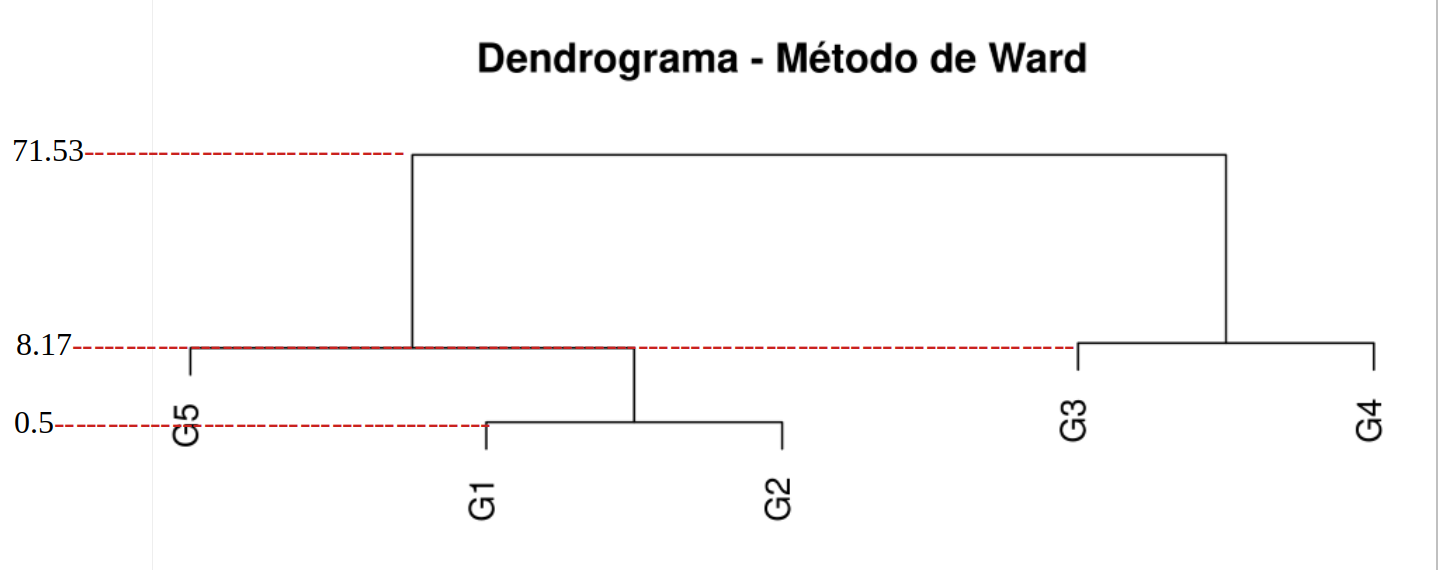
\includegraphics[width=0.8\textwidth]{../img/dendrograma.png}
        \caption{Dendrograma resultante. Imagen obtenida con R.}
    \end{figure}

\end{ejemplo}


\subsubsection{Métodos disociativos}

Como ya apuntamos al comienzo de la subsección, un método jerárquico \textit{disociativo} comienza con un único cluster constituido por todos los individuos
de nuestro conjunto de datos y lo divide en dos clusters. Sucesivamente, en cada iteración, uno de los clusters se divide en dos subclusters hasta conseguir
un cluster por elemento. \newline

Aunque la forma de calcular la distancia entre clusters es igual que en los aglomerativos, la diferencia está en que como se parte de un único cluster, se va
a intentar maximizar las distancias o, equivalentemente, minimizar las similitudes. En definitiva, lo que se persigue es separar los elementos más disímiles en 
clusters diferentes. \newline

Los métodos disociativos son generalmente de dos clases: \textit{monotéticos} y \textit{politéticos}. En un enfoque monotético, la división de un grupo en dos 
subgrupos se basa en una sola variable y resultan útiles cuando las variables son de tipo binario, mientras que el enfoque politético utiliza las $p$ 
variables para realizar la división. \newline

Tienen la misma desventaja que los aglomerativos: una vez realizada la partición, un elemento no puede trasladarse a otro grupo al que no pertenece en el momento 
de la partición. En cambio, si se buscan grupos más grandes, a veces se prefiere el enfoque disociativo al aglomerativo, en el que los grupos más grandes se alcanzan
solo tras un gran número de uniones de grupos más pequeños. A pesar de esto, son métodos mucho menos conocidos que los aglomerativos, de ahí que no haya tanta 
bibliografía acerca de ellos. \newline

Un aspecto fundamental en su aplicación es determinar el momento adecuado para parar la subdivisión de un cluster y empezar a fragmentar otro. Esto lo resuelve la 
variante del método propuesta por MacNaughton-Smith en el año 1964, diseñada especialmente para medidas de asociación positivas, y que presentamos formalmente
a continuación: \newline

Sea $C$ un cluster inicial. Definimos un subconjunto $S \subset C$ como el grupo fragmentado, y su complemento $R = C\backslash S$ como el resto del cluster. El 
proceso de división consistirá en evaluar, para cada elemento $x \in R$, la diferencia entre su disimilaridad promedio con los elementos de $R$ y su disimilaridad 
promedio con los elementos de $S$. \newline

La distancia promedio de un elemento $x$ respecto a un conjunto $A$ viene dada por: 
\[
d(x,A) = \frac{1}{n_{A}} \sum_{y\in A} d(x,y)
\]

donde $d(x,y)$ represeta la medida de disimilaridad entre los elementos $x$ e $y$.\newline

Para cada $x\in R$, calculamos:
\[
\Delta (x) = d(x,R) - d(x,S)
\]

Si existe un $x^{'} \in R$ tal que $\max_{x \in R}{\Delta (x)} > 0$, entonces $x^{'}$ se traslada a $S$. En caso contrario, el procedimiento se detiene y la división
se completa. \newline

\begin{nota}
    Podemos inicalizar el conjunto fragmentado $S$ con el elemento $x_{0} \in C$ que tenga la mayor disimilaridad promedio respecto a los demás elementos del cluster.
\end{nota}

%Para dividir un cluster, trabajamos con un grupo fragmentado y el resto. Buscamos el elemento del resto cuya distancia promedio (disimilaridad) con respecto a los demás
%elementos del resto, menos su distancia promedio con respecto a los elementos del grupo fragmentado sea mayor. Si la mayor diferenca es positiva, el elemento se
%traslada al grupo fragmentado. Si la mayor diferencia es negativa, el procedimiento se detiene y la división se completa. Podemos comenzar el grupo fragmentado con
%el elemento que tenga la mayor distancia promediio con respecto a los demás elementos del grupo.


\subsection{Métodos no jerárquicos} %Bib-1, Bib-2, Bejar-AC

Los \textit{métodos no jerárquicos} para el análisis cluster, también conocidos como métodos de partición, simplemente dividen los datos en un número predeterminado $k$
de clusters, donde no existe una relación jerárquica entre la solución con $k$ clusters y la de $(k+1)$, es decir, la solución con $k$ clusters no es el paso previo para
la solución con $(k+1)$. Esta es la principal diferencia con respecto a los jerárquicos, donde el número de clusters era desconocido a priori. \newline

En definitiva, dado un número $k$, buscamos particionar los datos en $k$ clusters de modo que los elementos dentro de cada cluster sean similares entre sí, mientras que los elementos 
de clusters distintos sean bastante diferentes\cite{Bib-1}\cite{Bib-2}.\newline

Se caracterizan por tener una estructura plana, es decir, no implican la construcción de una estructura jerárquica en forma de árbol, a diferencia de los métodos jerárquicos.
En su lugar, los elementos se asignan a los clusters directamente, teniendo en cuenta el número predefinido de clusters, $k$. No se sigue un proceso progresivo de combinación
o separación de grupos, como ocurre en los jerárquicos\cite{bejar-AC}. \newline

\begin{nota}
    Los algoritmos no jerárquicos son mucho más eficientes que los jerárquicos en términos computacionales.
\end{nota}

\subsubsection{Método \textit{k-means}}

El algoritmo \textit{k-means}, propuesto por MacQueen en el año 1967, es el método más popular entre los no jerárquicos. Debido a su extrema eficiencia, se usa con frecuencia en proyectos de
grandes dimensiones. Se denomina \textit{k-means} (k-medias) porque asigna cada individuo al cluster cuyo centroide esté más próximo, de entre $k$ clusters prefijados. Dicho centroide se calcula 
a partir de los elementos que conforman el cluster después de cada asignación, en lugar de hacerlo al final de cada ciclo, como ocurre en otros métodos, lo cual es un aspecto
clave de este algoritmo. \newline
Cabe resaltar que este algoritmo necesita acceso a los datos originales y permite mover los elementos de un cluster a otro, una reasignación que no está disponible en los métodos 
jerárquicos. \newline

Veamos cómo funciona el algoritmo: \newline

Sea $\mathcal{L} = \{x_{i} / i = 1,\dots,n\}$ el conjunto de puntos que conforman nuestro conjunto de datos y sea $k$ el número de clusters. Elegimos $k$ elementos que nos servirán de 
\textit{semillas}, las cuales se reemplazarán por los centroides de los clusters en el transcurso del algoritmo. Hay varias formas de elegir dichas semillas:
\begin{itemize}
    \item[(1)] Seleccionando $k$ elementos al azar, aunque quizás separados por una mínima distancia.
    \item[(2)] Eligiendo los $k$ primeros elementos del conjunto de datos, sujetos a una distancia mínima. 
    \item[(3)] Seleccionando los $k$ puntos más alejados entre sí en base a una medida de disimilaridad.   
\end{itemize}

entre otras opciones. \newline

Una vez elegidas las semillas, cada elemento de nuestro conjunto de datos se asignará al cluster que tenga la semilla más cercana, en términos de distancia euclidea. Una vez que 
un cluster pase a tener más de un elemento, se reemplaza la semilla por su centroide. Cuando todos los elementos hayan sido asignados, entonces nos plantemos si cada elemento está
más cerca del centroide del cluster donde está asignado o del de otro cluster. Esto es, calculamos el Error Cuadrático Medio (ECM) de cada observación con respecto al
centroide de su clúster actual y el resto de centroides:
\[
ECM = \sum_{j=1}^{k}\sum_{i_{C_{j}}}(x_{i_{C_{j}}}-\bar{x}_{j})^{'}(x_{i_{C_{j}}}-\bar{x}_{j})
\]

donde $\bar{x}_{j}$ es el centroide del $j$-ésimo cluster y $C_{j}$ es el cluster que contiene a $x_{i_{C_{j}}}$. \newline

Si está más cerca del centroide de otro cluster, dicho elemento se traslada a dicho cluster y se recalculan los centroides de ambos. El proceso continúa hasta 
que no se puedan hacer más mejoras en términos de error cuadrátrico medio (se persigue minimizar el ECM). \newline

Cabe destacar que este método es bastante sensible a la elección de las semillas al comienzo del mismo. Se aconseja probar con distintas semillas y analizar los resultados: si 
con diferentes elecciones de semillas se dan resultados muy diferentes, o se requieren demasiadas iteraciones para estabilizarse (convergencia lenta), podemos sospechar que los datos no 
forman grupos bien dfinidos de forma natural. \newline

También puede usarse como mejora de los métodos jerárquicos: se agrupan primero los elementos mediante un método jerárquico y luego, utilizando como semillas los centroides de estos grupos
aplicamos el algoritmo. De esta forma, podremos reasignar los puntos de un cluster a otro, en caso de necesitarlo. Suplimos así el handicap de los aglomerativos. \newline

Ofrecemos a continuación un ejemplo con el que ilustraremos el funcionamiento del método:

\begin{ejemplo}
    Supongamos que tenemos $8$ genotipos, $G_{1}, G_{2},\dots,G_{8}$, sobre los que observamos la expresión de dos genes, $A$ y $B$:

    \begin{table}[h]
        \centering
        \begin{tabular}{|c|c|c|}
            \hline
            \textbf{Genotipo} & \textbf{$A$} & \textbf{$B$} \\
            \hline
            $G_{1}$ & 2.5 & 2.7 \\
            \hline
            $G_{2}$ & 5.1 & 4.9 \\
            \hline
            $G_{3}$ & 2.8 & 3.2 \\
            \hline
            $G_{4}$ & 3.0 & 2.4 \\
            \hline
            $G_{5}$ & 8.3 & 3.3 \\
            \hline
            $G_{6}$ & 4.6 & 6.1 \\
            \hline
            $G_{7}$ & 9.3 & 4.6 \\
            \hline
            $G_{8}$ & 5.3 & 3.8\\
            \hline
            
        \end{tabular}
        \caption{Ejemplo método \textit{$k$-means}}

    \end{table}

    Queremos aplicar el método no jerárquico $k$-means para $k=3$. \newline

    Comenzamos eligiendo por semillas $3$ elementos aleatorios, $g_{i} = (a_{i},b_{i})$, $i=1,\dots,8$, de entre nuestro conjunto de datos. Estos
    serán los primeros centroides:
    \[
    \bar{g}_{C_{1}} = (3.0,2.4) \hspace{0.3cm} \bar{g}_{C_{2}} = (8.3,3.3) \hspace{0.3cm} \bar{g}_{C_{3}} = (4.6,6.1)
    \]

    Calculamos las distancias de todos los puntos de nuestro dataset a estos centroides y obtenemos:

    \begin{table}[h]
        \centering
        \begin{tabular}{|c|c|c|c|c|}
            \hline
            \textbf{$g_{i}$} & \textbf{$C_{1}$} & \textbf{$C_{2}$} & \textbf{$C_{3}$} & \textbf{Cluster más cercano}\\
            \hline
            $g_{1}$ & $0.5830952$ & $5.830952$ & $3.996248$ & $C_{1}$\\
            \hline
            $g_{2}$ & $3.2649655$ & $3.577709$  & $1.300000$ & $C_{3}$\\
            \hline
            $g_{3}$ & $0.8246211$ & $5.500909$ & $3.413210$ & $C_{1}$\\
            \hline
            $g_{4}$ & $0.0000000$ & $5.375872$ & $4.031129$ & $C_{1}$\\
            \hline
            $g_{5}$ & $5.3758720$ & $0.000000$ & $4.640043$ & $C_{2}$\\
            \hline
            $G_{6}$ & $4.0311289$ & $4.640043$ & $0.000000$ & $C_{3}$\\
            \hline
            $G_{7}$ & $6.6730802$ & $1.640122$ & $4.933559$ & $C_{2}$\\
            \hline
            $G_{8}$ & $2.6925824$ & $3.041381$ & $2.404163$ & $C_{3}$ \\
            \hline
            
        \end{tabular}
        \caption{Cálculo distancias respecto centroides}

    \end{table}

    A continuación, como todos los clusters han pasado de tener más de un elemento,$C_{1} = \{g_{1},g_{3},g_{4}\}$,
    $C_{2} = \{g_{5},g_{7}\}$, $C_{3} = \{g_{2},g_{6},g_{8}\}$, recalculamos los centroides:

    \[
    \bar{g}_{C_{1}} = (2.767,2.767) \hspace{0.3cm} \bar{g}_{C_{2}} = (8.80,3.95) \hspace{0.3cm} \bar{g}_{C_{3}} = (5.0,4.9333)
    \]

    Calculamos de nuevo las distancias de cada punto a los nuevos centroies para ver si hay que hacer alguna reasignación de algún punto
    a otro cluster:

    \begin{table}[h]
        \centering
        \begin{tabular}{|c|c|c|c|c|}
            \hline
            \textbf{$g_{i}$} & \textbf{$C_{1}$} & \textbf{$C_{2}$} & \textbf{$C_{3}$} & \textbf{Cluster más cercano}\\
            \hline
            $g_{1}$ & $0.2748737$ & $6.422811$ & $3.3522573$ & $C_{1}$\\
            \hline
            $g_{2}$ & $3.1615749$ & $3.820013$  & $0.1053987$ & $C_{3}$\\
            \hline
            $g_{3}$ & $0.4346136$ & $6.046693$ & $2.8007729$ & $C_{1}$\\
            \hline
            $g_{4}$ & $0.4346134$ & $6.003541$ & $3.2276321$ & $C_{1}$\\
            \hline
            $g_{5}$ & $5.5589767$ & $0.820061$ & $3.6820740$ & $C_{2}$\\
            \hline
            $G_{6}$ & $3.8042375$ & $4.718315$ & $1.2333649$ & $C_{3}$\\
            \hline
            $G_{7}$ & $6.7856876$ & $0.820061$ & $4.3128980$ & $C_{2}$\\
            \hline
            $G_{8}$ & $2.7359744$ & $3.503213$ & $1.1723348$ & $C_{3}$ \\
            \hline
            
        \end{tabular}
        \caption{Cálculo distancias respecto centroides}

    \end{table}

    Observamos que la asignación de puntos a clusters se mantiene constante con respecto al paso previo. Esto quiere decir que no es necesaria ninguna
    reasignación y, por tanto, que las asignaciones son definitivas. La agrupación la podemos ver en el siguiente gráfico:

    \begin{figure}[h]
        \centering
        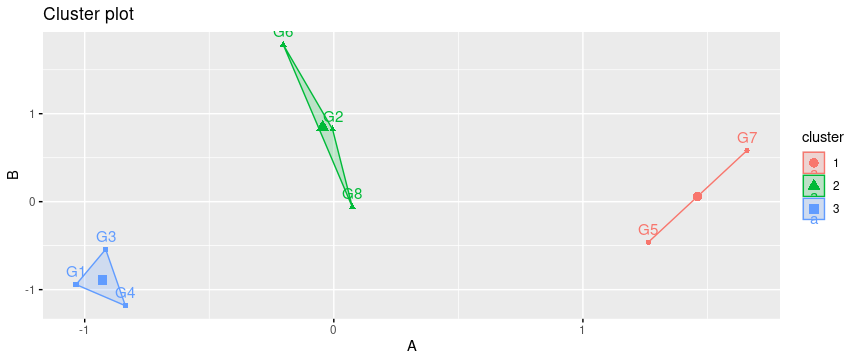
\includegraphics[width=0.8\textwidth]{../img/kmeans.png}
        \caption{Gráfico resultado final k-means. Imagen obtenida con R (ejemplo de elaboración propia).}
    \end{figure}
    
    
\end{ejemplo}

Por último, supongamos que hay elementos en nuestro conjunto de datos que podríamos catalogar como \textit{atípicos}, es decir, supongamos que tenemos \textit{outliers}. Estos valores, al 
ser muy dispares respecto a los demás, van a tener una gran influencia en el cálculo de los centroides, lo cual va a condicionar la agrupación. Esto lo podemos solucionar con el 
método $k$-menoids, que presentamos a continuación.

\subsubsection{Método \textit{$k$-medoids}}

El algoritmo \textit{$k$-medoids} se propone como una variante del método $k$-means que es mucho más robusta a ruidos y outliers. En lugar de 
usar el centroide como centro de un grupo, este algoritmo usa un punto real del grupo para representarlo; el \textit{medoide}, que es el objeto ubicado
más centralmennte en el grupo, y que minimiza la suma de disimilaridades respecto a los demás puntos, en lugar de la suma de los cuadrados de las distancias Euclideas. Aquí es donde
se refleja la robustez del método ante datos anómalos como los outliers. Pese a las ventajas evidentes que tiene el método, se ha visto que para conjuntos de 
datos muy grandes, la eficiencia del método se ve disminuida. \newline

El algoritmo comienza con la matriz de proximidad $D = (d_{ij})$, donde $d_{ij} = d(x_{i},x_{j})$, con $d$ una medida de disimilaridad, que nos la pueden dar de antemano o
bien la podemos calcular a partir del conjunto de datos, y una configuración inicial de los elementos en $k$ clusters. Usando la matriz $D$, podemos encontrar el elemento de 
cada cluster que minimiza la disimilaridad total con respecto a todos los elementos de su cluster (el menoide). Esto es, dado un cluster $C_{m}$, $m\in\{1,\dots,k\}$, se busca encontrar
un elemento $\bar{x}_{m}$ que haga mínima la suma $\sum_{i_{C_{m}}}d_(x_{i_{C_{m}}},\bar{x}_{m})$. \newline

Una vez hallados los medoides de los $k$ clusters, observamos la distancia de cada punto a los distintos medoides. Si existe un cluster $j$ de entre los $k$ que había prefijados que 
tiene algún elemento $x_{j}$ que está más cerca de otro medoide, entonces este elemento se reasigna al cluster de dicho medoide. Esta reasignación favorece a la minimización de la función
objetivo:
\[
d_{medoid} = \sum_{j=1}^{k}\sum_{i_{C_{j}}}d_(x_{i_{C_{j}}},\bar{x}_{j})
\]

A continuación se relocalizan medoides y se vuelven a reasignar los elementos. Se repite el proceso hasta que no haya reasignaciones que reduzcan 
el valor de la función objetivo.



\subsubsection{Determinación del número de clusters óptimo}

\newpage
\thispagestyle{empty}
\vspace*{\fill}
\begin{center}
    \large Parte III \\
    \vspace{0.5cm}           
    \LARGE \textbf{FUNDAMENTOS INFORMÁTICOS}
\end{center}
\vspace*{\fill}
\newpage


\chapter{Proyecto GEO (Gene Expression Omnibus)}

% esto ha salido de geo1, geo2, geo3

\textit{Gene Expression Omnibus} (GEO) es una base de datos pública e internacional gestionada por el Centro Nacional de Información 
Biotecnológica (NCBI) de la Biblioteca Nacional de Medicina (NLM) de EE.UU.
Está diseñada para almacenar y distribuir de manera libre conjuntos de datos relacionados con la expresión génica y otros estudios 
genómicos funcionales. Acepta tanto datos crudos como procesados, siempre con una descripción detallada del 
diseño experimental, las características de las muestras y las metodologías utilizadas en los estudios de genómica de alto rendimiento. \newline

Fue lanzada en el año 2000 debido al rápido crecimiento de los datos de expresión génica generados por tecnologías como los microarrays y la secuenciación 
de ADN. GEO ofrece una estructura abierta y flexible, que permite enviar, almacenar y acceder a conjuntos de datos muy variados, procedentes de 
técnicas como RNA-seq, single-cell RNA-seq (scRNA-seq), arrays de proteínas o tejidos, RT-PCR, estudios de metilación del genoma, análisis de 
variaciones en el número de copias (CNV) y más. Aunque aproximadamente el 90\% de los datos en GEO corresponden a estudios de expresión génica, 
su alcance se ha expandido con el tiempo. Actualmente, recibe datos de alrededor de 72 países, consolidándose como un recurso global, gratuito 
y de acceso público. \newline

Aunque no tiene como objetivo reemplazar bases de datos internas especializadas en expresión génica, GEO complementa estas fuentes actuando como 
un repositorio terciario\footnote[1]{Un repositorio terciario se refiere a un sistema que integra y organiza datos de diversas 
fuentes primarias y secundarias, sirviendo como un centro de distribución más amplio y accesible.} y centralizado. Su función principal es ofrecer una plataforma 
donde se difunden datos provenientes de múltiples estudios y fuentes, facilitando el acceso a información crucial para la investigación. Ofrece herramientas 
para la consulta, visualización y análisis de estos datos directamente desde su página web, lo que hace que sea fácil de usar incluso para investigadores 
sin experiencia en bioinformática o software especializado.\newline

Además, GEO sigue las normas establecidas por la \textit{Functional Genomics Data Society}, adhiriéndose a las directrices MIAME (\textit{Minimum Information About a Microarray Experiment}) 
y MINSEQE (\textit{Minimum Information about a high-throughput SEQuencing Experiment}), lo que asegura que los datos sean interpretables y reproducibles 
por la comunidad científica. Estas directrices definen los requisitos mínimos de información que debe acompañar a cada experimento, permitiendo 
su correcta interpretación, reutilización y comparación con otros estudios. \newline

En lo que sigue, iremos detallando los tres objetivos principales que persigue GEO y que son:

\begin{itemize}
    \item[1.] Proporcionar una base de datos robusta y verátil para almacenar de manera eficiente datos genómicos funcionales de alto rendimiento
    (véase Organizacón de los datos).
    \item[2.] Ofrecer prodemientos y formatos de envío sencillos que permitan a la comunidad científica depositar datos completos y bien antotados
    (véase Envío de datos).
    \item[3.] Facilitar mecanismos intuitivos que permitan a los usuarios consultar, localizar, revisar y descargar estudios y perfiles de expresión génica
    de interés (véase Navegación, descarga y consulta).
\end{itemize}


\section{Organización de los datos}

% esto ha salido del overview de GEO y de mi cabeza

La base de datos GEO almacena una amplia varidad de experimentos genómicos a gran escala, los cuales generan datos en muchos formatos, tipos de archivos
y contenido. Esto presenta un gran desafío en cuanto a manejo y consulta de la información. \newline

Es por ello por lo que ha sido diseñada con una estructura que permite adaptarse a esta diversidad de datos. Cabe señalar que los datos que vienen en tablas
no se almacenan de forma complementamente estructurada dentro de la base de datos central, sino que se guardan como tablas de texto plano, delimitadas por
tabulaciones, sin límites en cantidad de filas y columnas. \newline

Los registros que hay almacenados en GEO, todos ellos proporcionados por los investigadores (\textit{submitters}) se organizan de la siguiente forma:

\begin{itemize}
    \item \textit{Platforms: } son registros compuestos por:
    \begin{itemize}
        \item Una descripción general del array o del secuenciador.
        \item En el caso de las basadas en arrays,incluye además una tabla de datos que define la plantilla del array.
    \end{itemize} 

        Cada registro Platform recibe un número de acceso único y estable en GEO, con el prefijo \textit{GPLxxx} (por ejemplo, GPL570). \newline

        Puede estar referenciada por muchas muestras (Samples), las cuales pueden haber sido enviadas por múltiples remitentes (investigadores).

    \item \textit{Samples: } una muestra describe:
    \begin{itemize}
        \item Las condiciones bajo las cuales se manejó una muestra individual.
        \item Las manipulaciones a las que fue sometida.
        \item Un archivo original de datos en crudo o archivo de datos de secuenciación, procesados.
    \end{itemize}
    Al igual que antes, cada muestra tiene un Id asociado que comienza por \textit{GSMxxx}. \newline

    Una muestra debe referenciar a una y solo una Platform, que debe estar previamente definida, pero puede estar incluida en múltiples Series.
    
    \item \textit{Series: } un registro en serie:
    \begin{itemize}
        \item Vincula un grupo de muestras relacionadas (Samples).
        \item Sirve como punto central y descriptivo del estudio completo, ofreciendo una descripción en texto del experimento en su conjunto.
        \item Incluye un archivo comprimido (.tar) que contiene los archivos originales de datos en crudo o los archivos de datos de secuenciación
        procesados.
    \end{itemize}

    Cada serie recibe un identificador único que empieza por \textit{GSExxx}.
\end{itemize}

Como la estructura de la base de datos se organiza en torno a entidades bien definidas, como Platform, Sample y Serie, que poseen atributos específicos
y mantienen relaciones entre sí con cardinalidades reconocibles, es lógico pensar que el diseño conceptual de GEO está basado en un modelo entidad-relación
y, por ende, el lógico basado en el modelo relacional, que se obtiene a partir del conceptual mediante paso a tablas. \newline

Cabe señalar que los archivos de datos en crudo que acompañan a los registros se almacenan en un servidor FTP\footnote{FTP (\textit{FIle Transfer Protocol}) 
es un servicio utilizado para el envío y obtención de archivos entre dos equipos remotos} y están enlazados desde cada entrada. \newline

% referencia FTP: https://blog.infranetworking.com/servidor-ftp/ 

En base a toda esta información acerca de las entidades involucradas y sus relaciones, podemos construir un posible diagrama E/R para esta base de datos:

\begin{figure}[h]
    \centering
    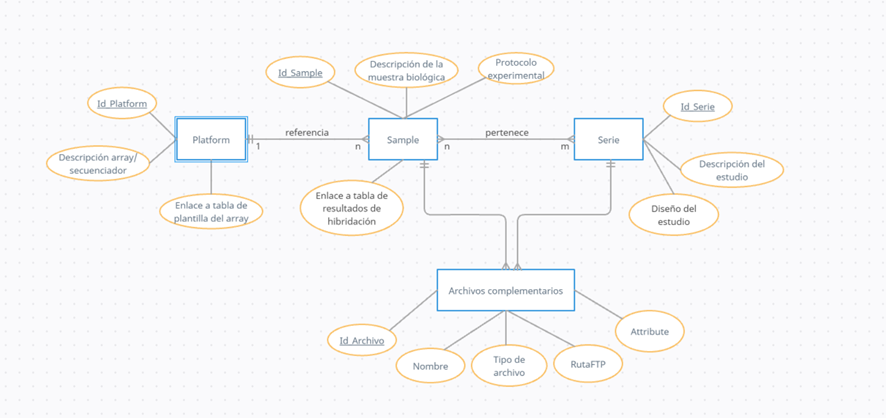
\includegraphics[width=1\textwidth]{../img/diagramaER.png}
    \caption{Diagrama Entidad-Relación (Fuente: elaboración propia).}
\end{figure}


% a lo mejor esto lo pongo en una sección a parte. Tendría que cambiar la introducción.
% esto ha salido del overview de GEO y de geo3.pdf

Por otra parte, los datos de \textit{Platform}, \textit{Sample} y \textit{Series} que envían los investigadores a GEO son bastante diversos en cuanto a formato, 
contenido y nivel de detalle con el que se describen los experimentos. Sin embargo, a pesar de estas diferencias, todas las presentaciones de estudios de expresión 
génica basados en arrays comparten una serie de elementos comunes:

\begin{itemize}
\item Información para identificar la secuencia de cada elemento presente en la \textit{Platform}. Es decir, cada sonda o fragmento de secuencia está asociado a 
una secuencia de nucleótidos específica, lo que permite localizarla de forma única y vincularla a un gen o región concreta del genoma.
\item Mediciones de expresión normalizadas incluidas en las tablas de \textit{Sample}.
\item Una descripción textual que recoge de dónde procede la muestra biológica y cuál es el objetivo del estudio.
\end{itemize}

Para organizar toda esta información y facilitar su consulta y análisis, se lleva a cabo un proceso que combina extracción automatizada de datos con una revisión 
manual, conocida como \textit{curación de datos}\footnote{La curación manual consiste en una revisión realizada por personal especializado que garantiza la calidad, 
consistencia y coherencia de los datos recopilados, corrigiendo posibles errores y asegurando que se ajustan a los estándares establecidos.}. Gracias a este procedimiento, 
los datos enviados por los investigadores se reorganizan en registros más estructurados y accesibles denominados \textit{DataSets}. \newline

Un \textit{DataSet} agrupa un conjunto de muestras biológicas que son comparables entre sí desde un punto de vista biológico y estadístico, y que pertenecen a una 
misma \textit{Platform}. Esto significa que todas comparten el mismo conjunto de sondas o elementos en el array, y que las mediciones de expresión se han procesado 
aplicando criterios homogéneos de normalización y ajuste de fondo. De esta forma, se asegura que los valores se puedan comparar de forma adecuada. \newline

Además, a partir de estos \textit{DataSets} se generan los denominados \textit{Profiles}. Un \textit{Profile} consiste en las mediciones de expresión de un gen concreto 
a lo largo de todas las muestras incluidas en un \textit{DataSet}. Estos perfiles permiten estudiar cómo varía la expresión de un gen específico en diferentes condiciones 
experimentales o tipos de muestra, y se pueden consultar mediante la herramienta \textit{GEO Profiles}, que ofrece opciones de búsqueda y visualización específicas para 
este tipo de datos. Todos ellos se indexan en la base de datos \textit{Entrez GEO Profiles}. \newline

Es importante señalar que no todos los registros \textit{Series} que se envían a GEO acaban formando parte de un \textit{DataSet}. Este trabajo de selección y reorganización 
lo realiza el personal encargado de la curación y mantenimiento de la base de datos, que se encarga de elegir qué estudios reúnen las condiciones necesarias para integrarse 
en un \textit{DataSet}. Además, los \textit{DataSets} y \textit{Profiles} son la base para muchas de las herramientas de visualización y análisis que ofrece GEO, como los 
gráficos de perfiles de expresión génica o los clústeres de agrupación de muestras. Por último, cada \textit{DataSet} recibe un identificador único y estable con el prefijo 
\textit{GDS}, y se pueden consultar desde la interfaz \textit{Entrez GEO DataSets}.

\begin{figure}[h]
    \centering
    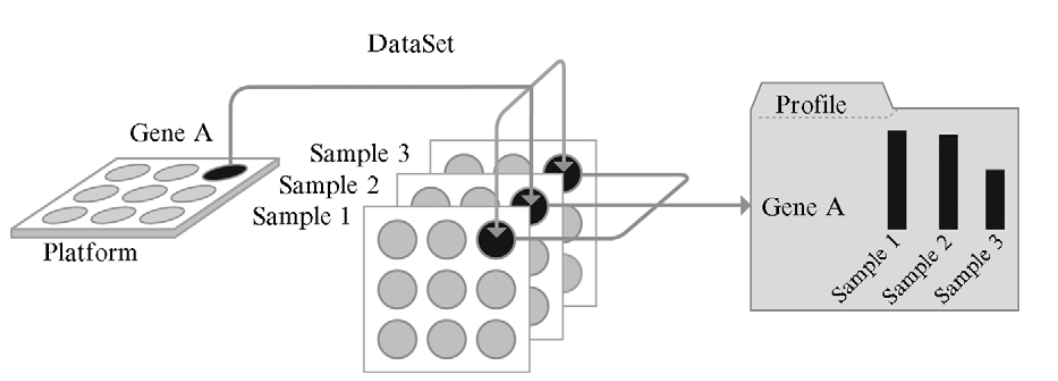
\includegraphics[width=1\textwidth]{../img/geo-datasets.png}
    \caption{Relación entre Platforms, Samples, DataSets y Profiles (Fuente: ).}  % geo-4.pdf
\end{figure}

% referencia curación manual:  https://es.wikipedia.org/wiki/Curaci%C3%B3n_de_datos

\section{Envío de datos}

% esto lo estoy viendo de geo4.pdf

Como se adelantó en la introducción, la base de datos GEO se adhiere a las reglas establecidas en MIAME y, por consiguiente, el envío de los procedimientos promueven
su cumplimiento. Sin embargo, es el propio investigador el que tiene la responsabiilidad, en última instancia, de asegurar que los datos estén suficientemente anotados y
que se cumple la normativa para investigación con sujetos humanos. A contininuación se va a hacer un desglose de los pasos de los que se compone el flujo de datos que siguen 
los investigadores al enviar datos a GEO:

\begin{itemize}
    \item[1.] \textit{Inicio del depósito de datos:} Los investigadores envían sus datos a GEO antes de enviar su manuscrito a una revista. Esto lo hacen a través de su cuenta en 
    de MyNCBI.
    \item[2.] \textit{Formatos de envío:} GEO permite varios formatos de envío, como hijas de cálculo o XML, según las instrucciones de envío.
    \item[3.] \textit{Valiidación y curación:} Los envíos pasan primero porr una validación sintáctica automática. Luego, un curador de GEO revisa que los datos estén bien organizados
    y contengan suficente información. Si hay algún problema, el curador colabora con los autors hasta resolverlos.
    \item[4.] \textit{Asignación de identificadores:} Cuando todo está correcto, se asignan números de acceso estables que se pueden citar en el manuscrito.
    \item[5.] \textit{Privacidad previa a la publicación:} Los datos se mantienen privados hasta que el artículo es publicado. Durante ese tiempo, los autores pueden generar una URL
    que de acceso conficencial a editores y revisores.
    \item[6.] \textit{Disponibilidad pública e indexación:} Tras su publicación, los datos de Platform, Sample y Serie se indexan en la base de datos \textit{Entrez GEO DataSets}, donde
    los usuarios pueden consultar y descargar los datos, o realizar un análisi de expresión génica mediante la herramienta de comparación \textit{GEO2R}.
    \item[7.] \textit{Interoperabilidad con otras bases de datos:} Alguna partes del envío se transiferen a otras bases de datos como \textit{SRA} (para secuencias) o \textit{BioProject}
    (para descripciones de estudios), con enlaces recíprocos hacia GEO.
    \item[8.] \textit{Curación mensual adicional:} Cada mes, algunas Series se seleccionan para una curación más profunda, creando \textit{GEO DataSets} y \textit{GEO Profiles}, derivados 
    de estos.
    
\end{itemize}

\section{Navegación, descarga y consulta}


\subsection{Navegación}
% https://www.ncbi.nlm.nih.gov/geo/browse/

El navegador de repositorios GEO cuenta con pestañas que contienen tablas donde se listan los registros de Series, Samples, Platforms y DataSets. Las tablas incluyen informaciión que se 
puede buscar y filtrar, así como enlaces a registros relacionados y descargas de archivos complementarios. Estas tablas se pueden exportar e incluyen información adicional que no se muestra
en el navegador, como identificadores de \textit{PubMed} y accesiones relacionadas en SRA.

\begin{figure}[h]
    \centering
    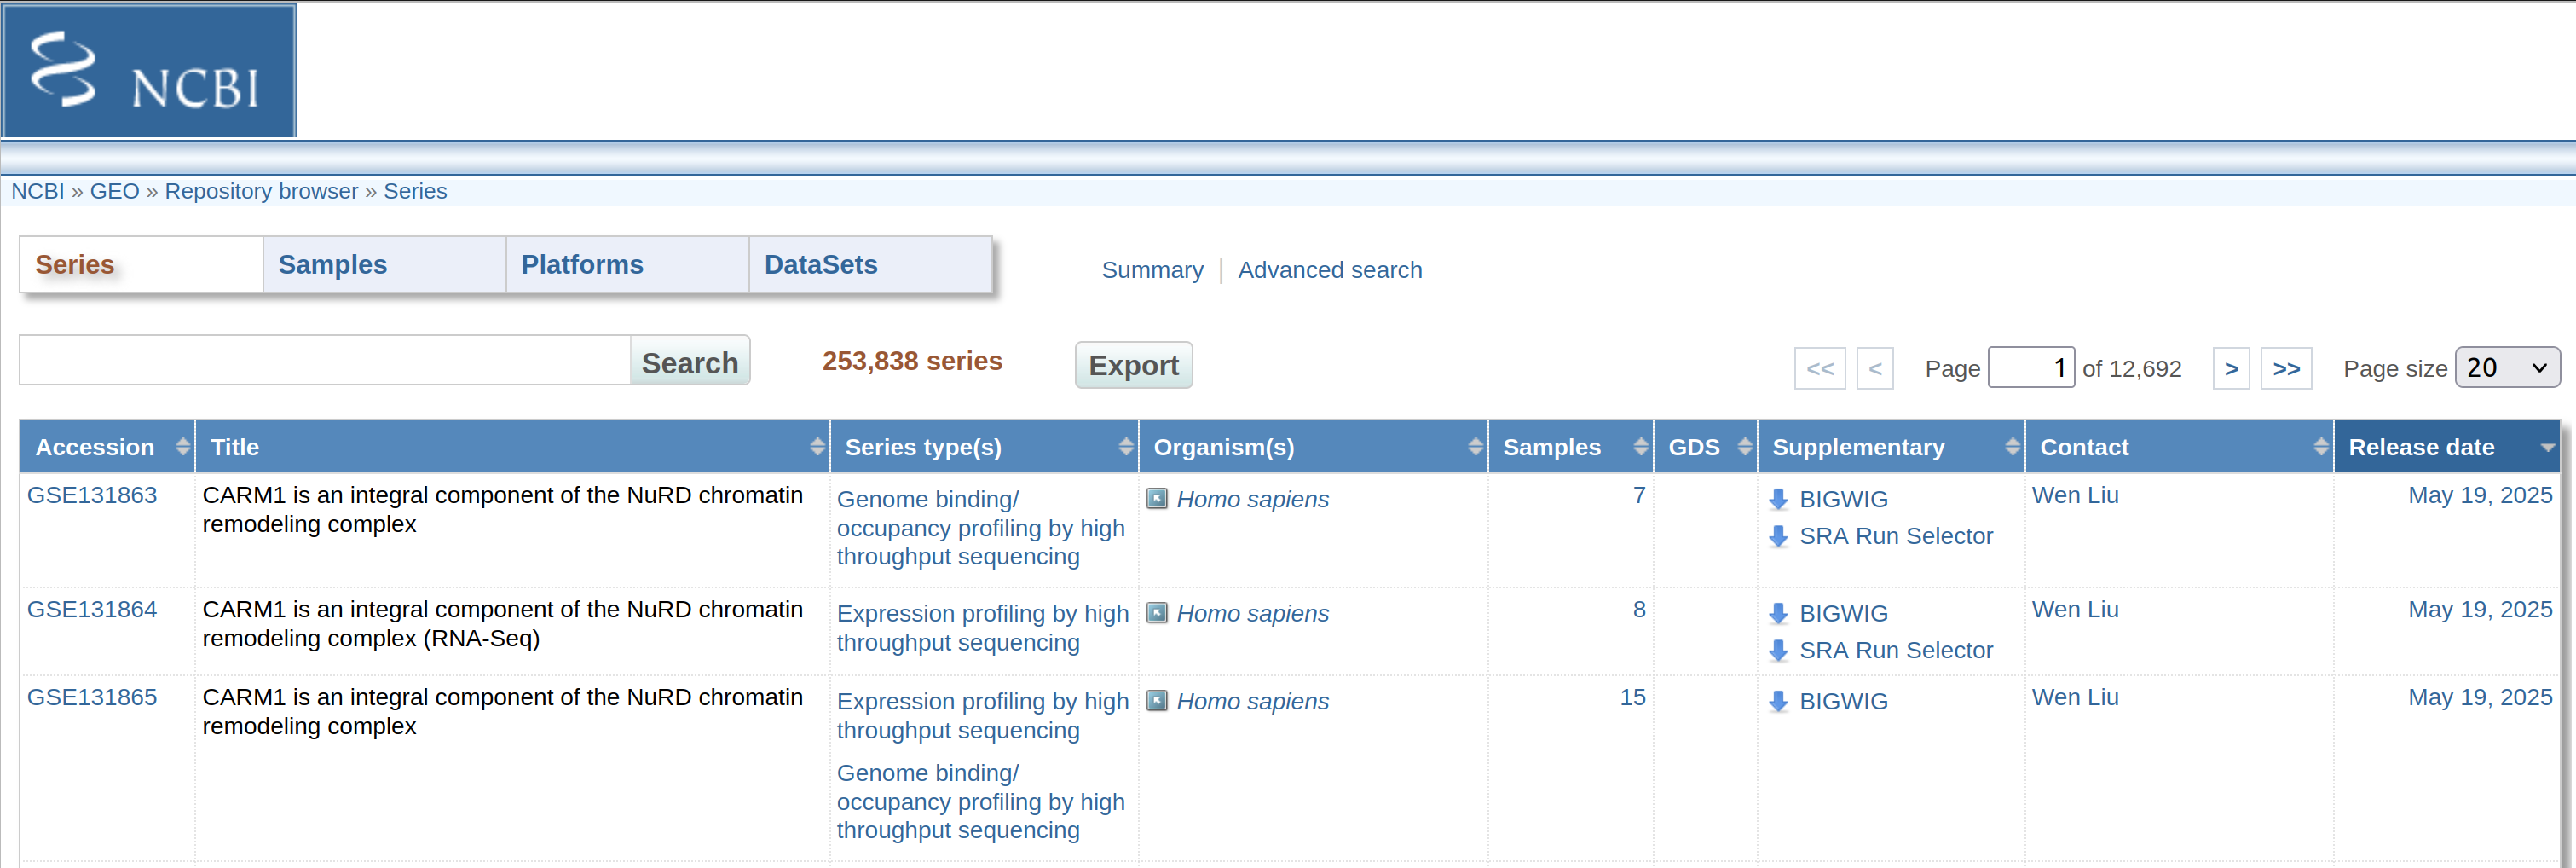
\includegraphics[width=1\textwidth]{../img/geo-browser.png}
    \caption{Navegador GEO (Fuente: ).}
\end{figure}

\subsection{Descarga de datos}

Todos los datos almacenados en GEO pueden descargarse en una gran variedad de formatos usando varios mecanismos que se presentan a continuación.

Para descargar registros GEO originales podemos hacerlo de cualquiera de las siguientes formas:

\begin{itemize}
    \item \textit{Enlaces a registros de Series:} Al pie de cada registro Serie de GEO, figuran enlaces a descargas de familias de experimentos en diversos formatos y archivos complementarios.
    Estos archivos están comprimidos con gzip (extension .gz o .tgz). Para descomprimir y leer estos archivos, se ha de utilizar la herramienta \textit{WinZip} o \textit{7-Zip}.
    \item \textit{Descarga FTP:} Todos los registros GEO y los archivos de datos en crudo pueden descargarse gratuitamente desde el sitio FTP de GEO. Sin embargo, GEO contiene a día de hoy tal
    cantidad de envíos que ya no se puede acceder a algunos directorios principales mediante navegadores web debido a errores de latencia. En tales casos, es necesario pasar por alto el directorio 
    principal e ir directamente al directorio de destino. Por ejemplo, para la serie \textit{GSE1000}:

    \[
        ftp://ftp.ncbi.nlm.nih.gov/geo/series/GSE1nnn/GSE1000/matrix/ 
    \]
    
    La mayoría de los archivos del servidor FTP están comprimidos con gzip (extensión .gz y .tgz). Para descomprimirlos y leerlos, si se usa Windows, se puede hacer con WinZip o 7-Zip. Si se dispone 
    de UNIX, se deberán de seguir los comandos tar y gunzip para extraer los archivos, por ejemplo: \newline

    \begin{lstlisting}[language=bash, backgroundcolor=\color{lightgray}, basicstyle=\ttfamily, keywordstyle=\color{blue}, numbers=none]
    $ tar -xf GSExxxx_RAW.tar
    $ gunzip *gz \end{lstlisting}
        
    \item  \textit{Barra de visualización por identificadores (\textit{Accessions}):} Se encuentra en la parte superior de cada registro GEO y puede utilizarse para descargar o visualizar registros completos o parciales,
    Platforms, Samples y Series relacionados. La función \textit{Scope} (el alcance) permite visualizar un único número de acceso (\textit{Self}), cualquiera (\textit{Platform, Sample o Serie}),
    o todos (\textit{Family}) los registros relacionados con el acceso especificado (el identificador que hayamos puesto). \textit{Amount} determina la cantiad de datos mostrados con opciones que incluyen 
    sólo metadatos (\textit{Brief}), metadatos y las 20 primeras filas de la tabla de datos (\textit{Quick}), sólo tabla de datos (\textit{Data}) o registros completos de metadatos/tabla de datos (\textit{Full}). 
    \textit{Format} controla si los registros se muestran en formato HTML, SOFT (texto sin formato) o MINiML (XML).

    \begin{figure}[h]
        \centering
        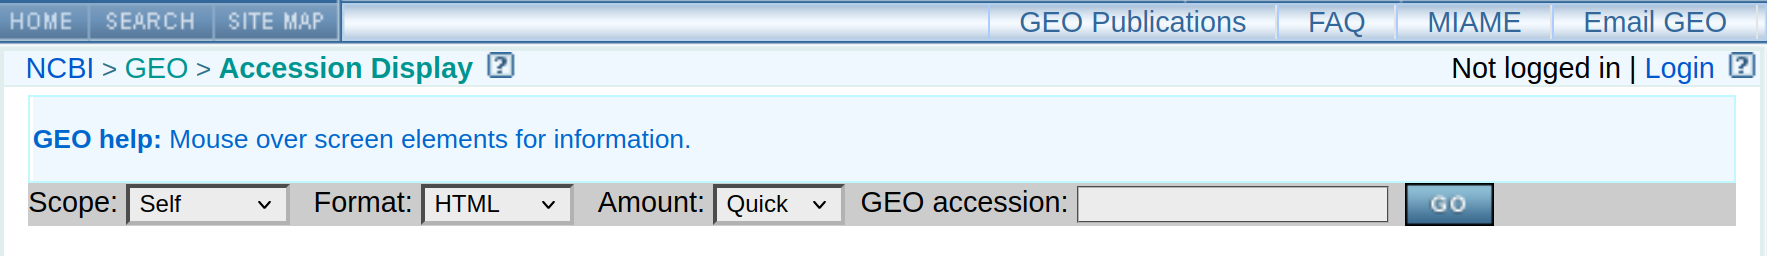
\includegraphics[width=1\textwidth]{../img/geo-displayBar.png}
        \caption{Barra de navegación de accesiones (Fuente: ).}  % https://www.ncbi.nlm.nih.gov/geo/query/acc.cgi
    \end{figure}
    \item \textit{Construcción de una URL:} Una forma alternativa de usar la barra de visualización de accesos anteriormente descrita, es construir una URL para devolver los datos que nos interesen. Las URLs 
    tienen el siguiente formato: 

    
    \url{https://www.ncbi.nlm.nih.gov/geo/query/acc.cgi?acc=gpl96&targ=self&view=brief&form=text}


    Esta URL, bajo el esquema http y la autoridad \textit{www.ncbi.nlm.nih.gov}, accederá a \textit{acc.cgi} a través de la ruta \textit{geo/query/acc.cgi} y realizará una consulta para devolver un fichero de 
    texto que contiene una breve vista de la accesión \textit{GPL96}. \newline  % partes de una URI tema 1 PW

    Los posibles valores para las componentes de la consulta son:

    \begin{itemize}
        \item \textit{acc} = un identificador GEO válido, según el formato \textit{glpxxx, gsmxxx} o \textit{gsexxx}.
        \item \textit{targ} = \textit{self, gsm, gpl, gse} o \textit{all}.
        \item \textit{view} = \textit{brief, quick, data} o \textit{full}.
        \item \textit{form} = \textit{text, html} o \textit{xml}.
    \end{itemize}

    \item \textit{Descargas de consultas en Entrez GEO DataSets:} Todos los registros originales pueden buscarse y descargarse a través de la interfaz \textit{Entrez GEO DataSets.} Los resultados pueden exportarse
    configurando la barra de herramientes de la parte superior de la página como \textit{'Enviar a: Archivo'}.
        
\end{itemize}


Para descargar \textit{DataSets} y \textit{Profiles} curados, podemos usar:

\begin{itemize}
    \item \textit{Enlaces en DataSets}: Los enlaces a los archivos \textit{SOFT} de \textit{DataSet} están disponibles en el botón <<download>> de cada registro de \textit{DataSet}. Estos archivos están comprimidos
    con gzip.
    \item \textit{Descarga FTP:} Todos los registros \textit{GEO DataSet} están disponibles, como hemos dicho antes, en el servidor FTP de GEO.
    \item \textit{Valores de Perfil:} Para descargar datos de perfil, usamos el botón \textit{Download profile data} situado en la parte superior de las páginas de recuperación de 
    \textit{Entrez GEO Profiles} para descargar los valores de expresión de los genes encontrados en la consulta.
    \item \textit{Descargas de consultas a Entrez GEO DataSets y Entrez GEO Profiles:} Es posible exportar resúmenes de documentos de \textit{Entrez GEO DataSets} y \textit{Entrez GEO Profiles} configurando la barra
    de herramientas de la cabecera de la página como \textit{'Enviar a: Archivo'}.
\end{itemize}

\subsection{Consulta de datos}

% se ha sacado de geo3.pdf 

NCBI dispone de un potente sistema de búsqueda y recuperación llamado \textit{Entrez}, que permite consultar el contenido de su red de bases de datos integradas. Los datos de GEO están disponibles en dos bases de
datos independientes a las que ya hemos hecho referencia en numerosas ocasiones: \textit{Entrez GEO DataSets} y \textit{Entrez GEO Profiles}. \newline

El flujo de trabajo habitual consiste en que el usuario primero identifique estudios de interés mediante la búsqueda en \textit{Entrez GEO DataSets}, y posteriormente utilice \textit{GEO2R} o \textit{GEO Profiles} para
localizar genes específicos o patrones de expresión génica dentro de ese estudio. Tambiéen es posible consultar directamente \textit{Entrez GEO Profiles}. \newline

Además, \textit{Entrez} genera numerosos enlaces que conectan datos relacionados: enlaces entre bases de datos que vinculan GEO con otros recursos de NCBI como \textit{PubMed}, \textit{GenBank} o \textit{Gene}; y enlaces
dentro de la propia base de datos, que conectan genes relacionados por patrón de expresión, posición cromosómica o secuencia. \newline

Ambas bases de datos permiten refinar búsquedas mediante filtros por campos específicos, búsqueda por facetas, que sería la forma más sencilla de consulta, y consultas avanzadas combinadas. \newline

Veamos cómo se puede consultar la base de datos \textit{Entrez GEO DataSets} mediante consultas avanzadas. Como ya se ha mencionado anteriormente, esta base de datos almacena las descripciones originales de los registros de Platform, Sample y Series
aportados por los autores, así como los \textit{DataSets} curados. Puede buscarse utlizando distintos atributos como palabras clave, organismo, tipo de estudio o autores. 

\begin{figure}[h]
    \centering
    
\includegraphics[width=1\textwidth]{../img/geo-datasets-browser.png}
    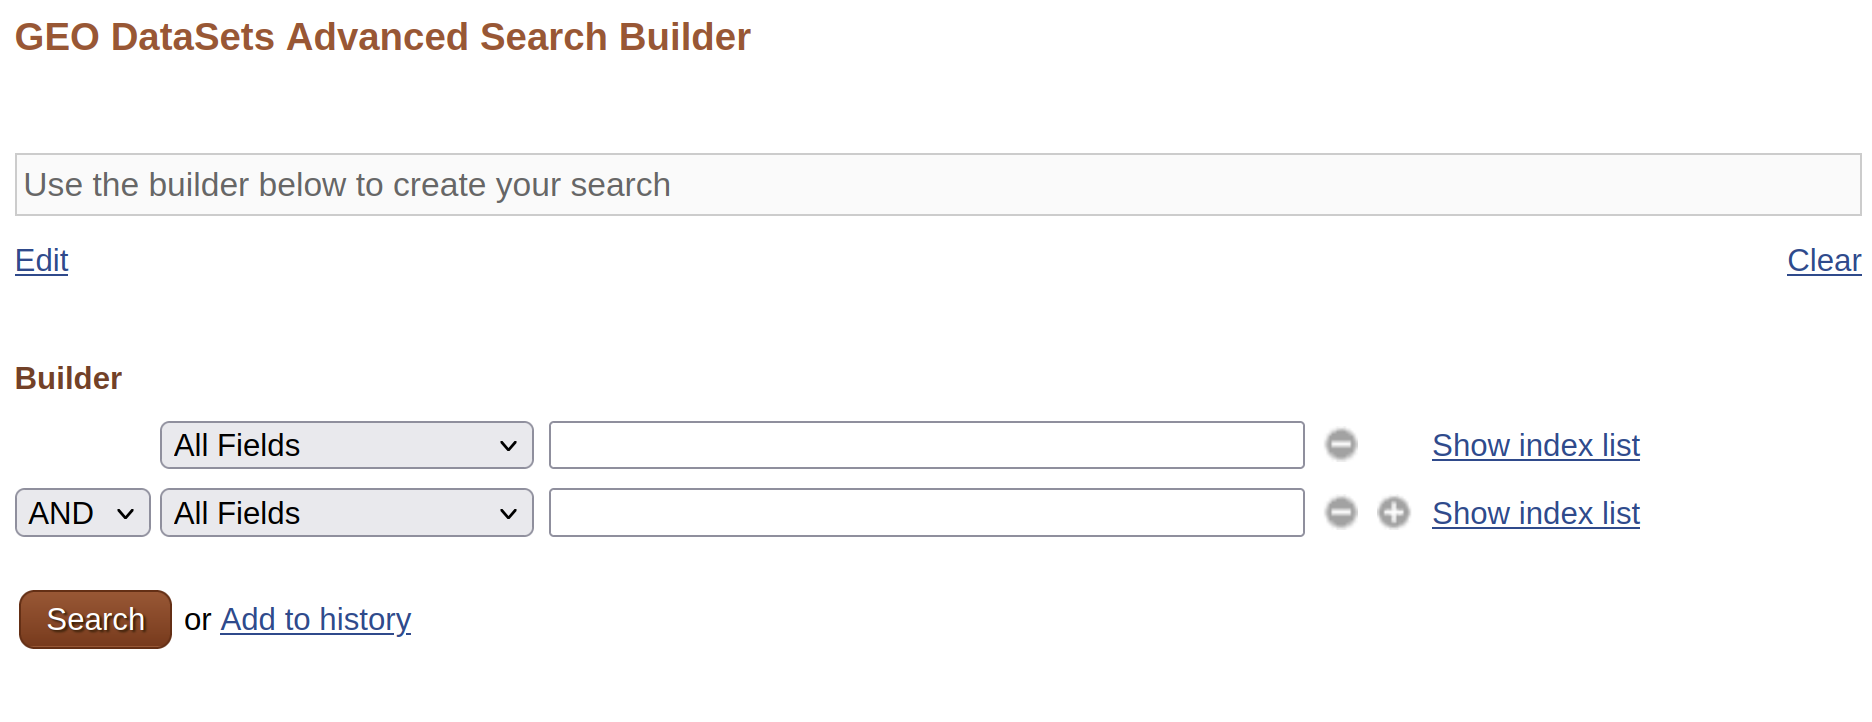
\includegraphics[width=1\textwidth]{../img/geo-adv-queryDataset.png}
    \caption{Construcción de consulta avanzada en \textit{Entrez GEO DataSets} (Fuente: ).}  % https://www.ncbi.nlm.nih.gov/gds/advanced
\end{figure}

Algunos ejemplos de consultas serían:

\begin{itemize}
    \item Recuperar estudios que investigan el efecto del tabaco o la dieta en mamíferos no humanos:
    \begin{lstlisting}[basicstyle=\ttfamily\small, backgroundcolor=\color{lightgray}, numbers=none, aboveskip=0pt, belowskip=0pt]
(smok* OR diet) AND (mammals[organism] NOT human[organism])\end{lstlisting}

    \item Buscar estudios que analicen expresión génica mediante secuenciación de nueva generación:
    \begin{lstlisting}[basicstyle=\ttfamily\small, backgroundcolor=\color{lightgray}, numbers=none, aboveskip=0pt, belowskip=0pt]
"expression profiling by high throughput sequencing"[DataSet Type]\end{lstlisting}

    \item Recuperar envíos que incluyan archivos Affymetrix CEL:
    \begin{lstlisting}[basicstyle=\ttfamily\small, backgroundcolor=\color{lightgray}, numbers=none, aboveskip=0pt, belowskip=0pt]
cel[Supplementary Files]\end{lstlisting}

    \item Localizar DataSets curados que incluyan 'edad' como variable experimental:
    \begin{lstlisting}[basicstyle=\ttfamily\small, backgroundcolor=\color{lightgray}, numbers=none, aboveskip=0pt, belowskip=0pt]
age[Subset Variable Type]\end{lstlisting}

    \item Consultar estudios que contengan entre 100 y 500 muestras:
    \begin{lstlisting}[basicstyle=\ttfamily\small, backgroundcolor=\color{lightgray}, numbers=none, aboveskip=0pt, belowskip=0pt]
100:500[Number of Samples]\end{lstlisting}

    \item Buscar estudios en los que aparezca ‘Smith, A.’ como autor:
    \begin{lstlisting}[basicstyle=\ttfamily\small, backgroundcolor=\color{lightgray}, numbers=none, aboveskip=0pt, belowskip=0pt]
smith a[Author]\end{lstlisting}

\end{itemize}

Por su parte, como ya se mencionó anteriormente, la base de datos \textit{Entrez GEO Profiles}, almacena perfiles de expresión génica derivados de \textit{DataSets} curados de GEO.
Cada perfil se muestra como un gŕafico que representa el nivel de expresión de un gen a lo largo de todas las muestras de un \textit{DataSet}. En la parte inferior del bráfico hay unas
barras que indican el contexto experimental, lo que permite ver fácilmente si un gen está diferencialmente expresado en distintas condiciones. \newline

\begin{figure}[h]
    \centering
    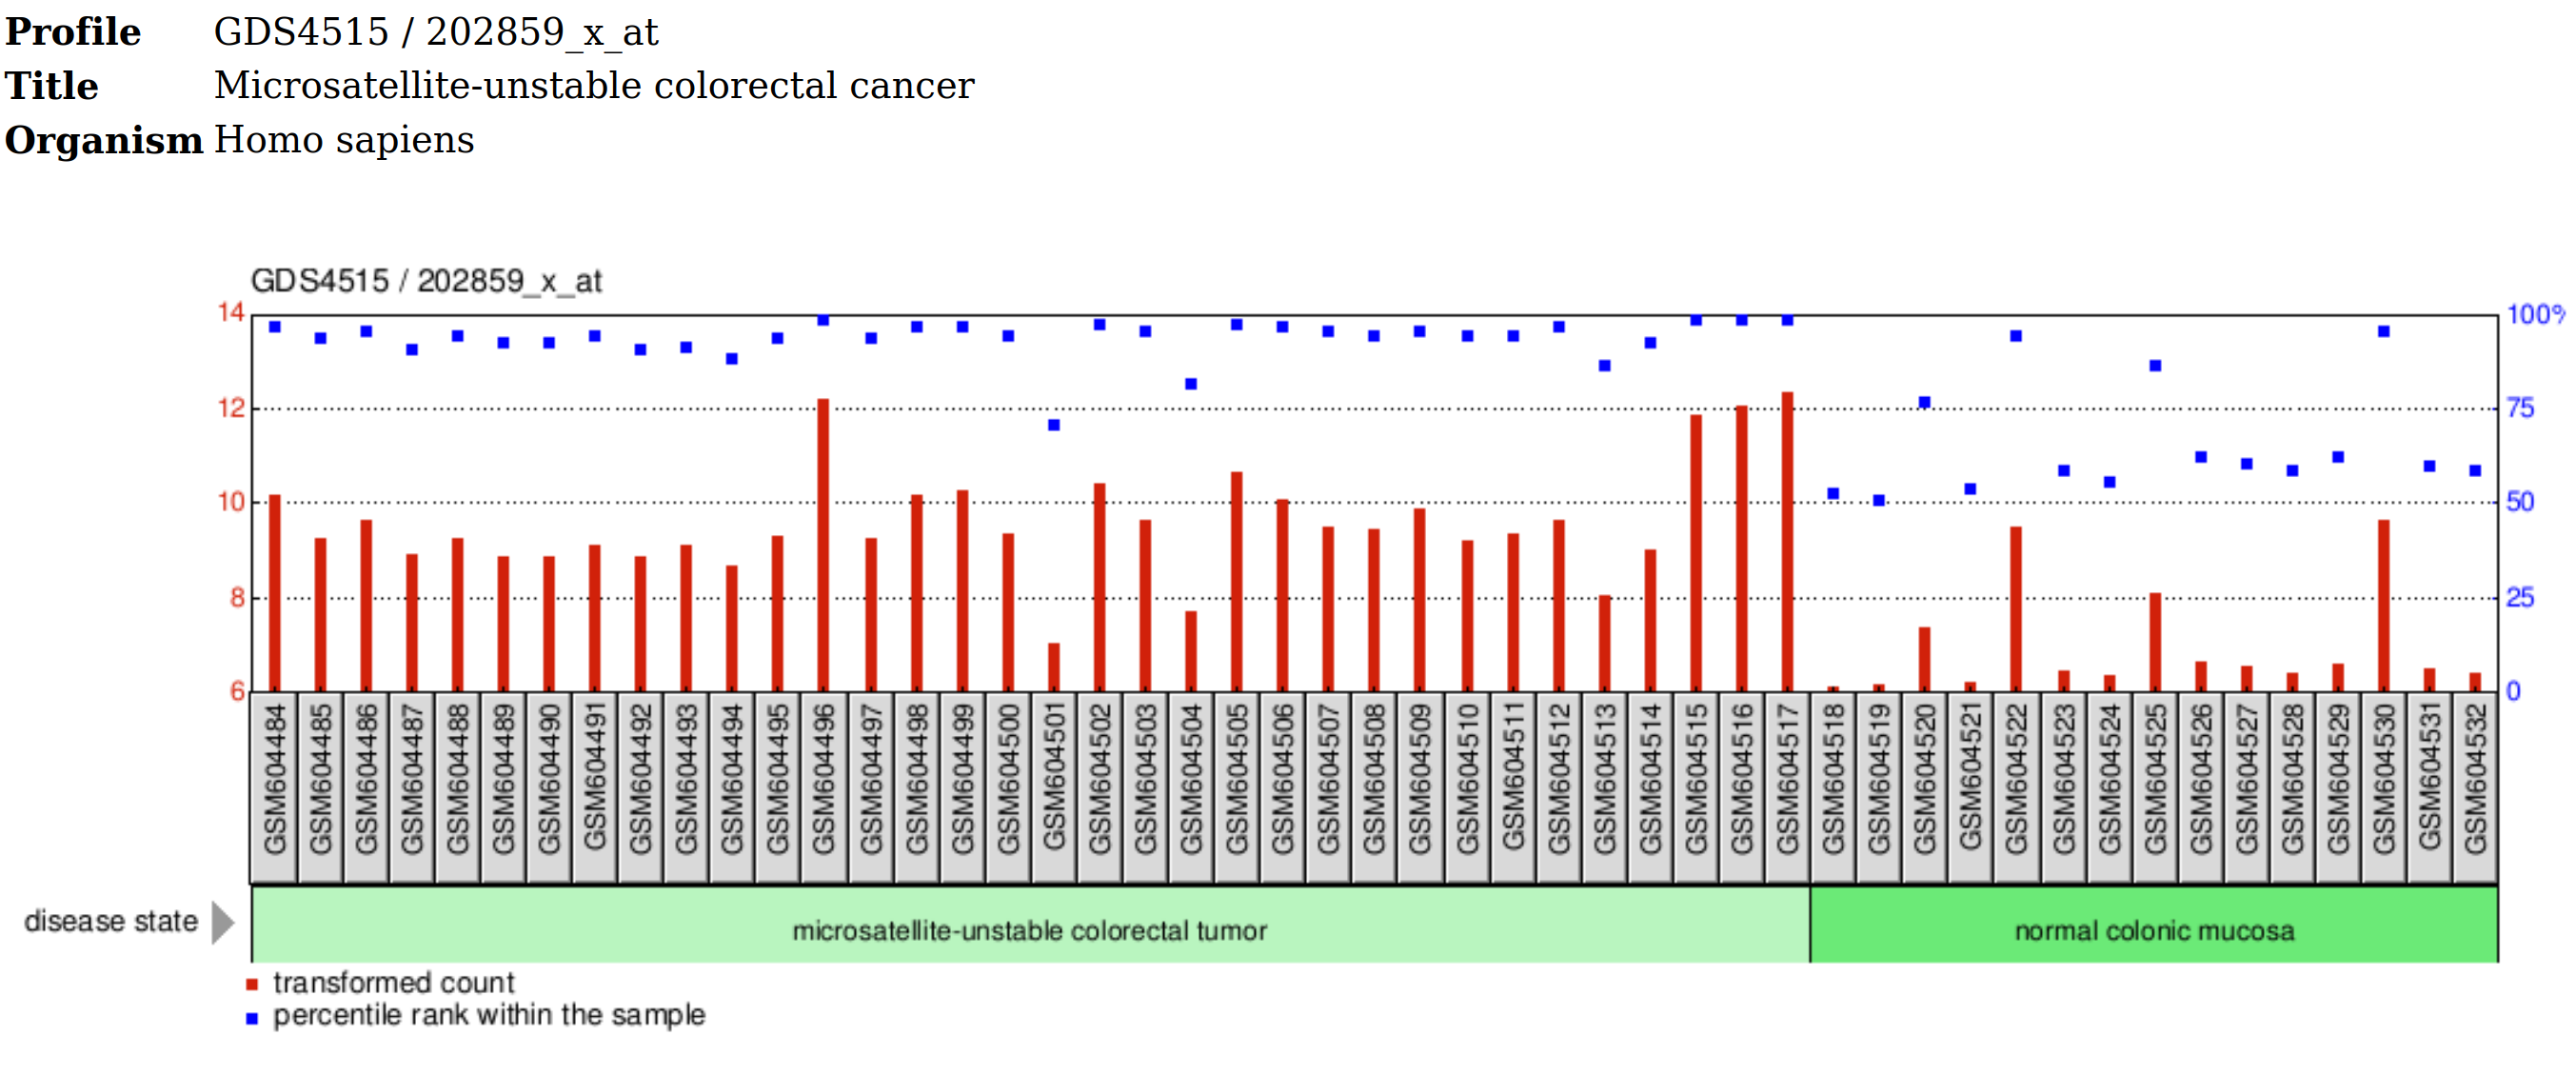
\includegraphics[width=1\textwidth]{../img/geo-profile.png}
    \caption{Ejemplo de perfil (Fuente: ).}  % https://www.ncbi.nlm.nih.gov/geo/tools/profileGraph.cgi?ID=GDS4515:202859_x_at
\end{figure}

Se puede consultar usando diferentes atributos, como palabras clave, símbolos o nombres de genes, identificadores de \textit{GenBank} o perfiles que estén marcados como diferencialmente expresados.
Algunos ejemplos de consultas incluyen:

\begin{itemize}
    \item Recuperar todos los perfiles de expresión génica para CYP1A1:
    \begin{lstlisting}[basicstyle=\ttfamily\small, backgroundcolor=\color{lightgray}, numbers=none, aboveskip=0pt, belowskip=0pt]
CYP1A1[Gene Symbol]\end{lstlisting}

    \item Recuperar perfiles de expresión génica de CYP1A1 o ME1 en DataSets que investiguen los efectos del tabaco o la dieta:
    \begin{lstlisting}[basicstyle=\ttfamily\small, backgroundcolor=\color{lightgray}, numbers=none, aboveskip=0pt, belowskip=0pt]
(CYP1A1[Gene Symbol] OR ME1[Gene Symbol]) AND (smok* OR diet)\end{lstlisting}

    \item Recuperar perfiles para todas las quinasas en el DataSet con número de accesión GDS182:
    \begin{lstlisting}[basicstyle=\ttfamily\small, backgroundcolor=\color{lightgray}, numbers=none, aboveskip=0pt, belowskip=0pt]
kinase[Gene Description] AND GDS182\end{lstlisting}

    \item Recuperar perfiles para genes que tengan el término Gene Ontology (GO) ‘apoptosis’ en el DataSet con accesión GDS182:
    \begin{lstlisting}[basicstyle=\ttfamily\small, backgroundcolor=\color{lightgray}, numbers=none, aboveskip=0pt, belowskip=0pt]
apoptosis[Gene Ontology] AND GDS182\end{lstlisting}

    \item Recuperar perfiles de genes que se encuentren dentro del rango 10000:3000000 en el cromosoma 8 de ratón:
    \begin{lstlisting}[basicstyle=\ttfamily\small, backgroundcolor=\color{lightgray}, numbers=none, aboveskip=0pt, belowskip=0pt]
(8[Chromosome] AND 10000:3000000[Base Position]) AND mouse[organism]\end{lstlisting}

    \item Recuperar genes que muestran expresión diferencial en DataSets que examinan el efecto de un agente:
    \begin{lstlisting}[basicstyle=\ttfamily\small, backgroundcolor=\color{lightgray}, numbers=none, aboveskip=0pt, belowskip=0pt]
agent[Flag Information] AND "value subset effect"[Flag Type]\end{lstlisting}
\end{itemize}


Tras haber explorado en detalle la base de datos GEO, la organización de los datos y las herramientas de descarga y consulta, en la siguiente sección nos centraremos en \textit{Bioconductor}, un conjunto de paquetes de software en R 
diseñado para el análisis e interpretación de datos genómicos. Veremos cómo Bioconductor permite aprovechar al máximo la información obtenida de GEO mediante potentes técnicas estadísticas y bioinformáticas.

\newpage

\chapter{Bioconductor}  % referencias: https://bioconductor.org/about/ https://bioinformatics.ccr.cancer.gov/docs/rintro/Lesson_8/, bioconductor-2.pdf, bioconductor-1.pdf


Bioconductor es un proyecto de código abierto y un repositorio de paquetes para R que se usa mucho en bioinformática y biología computacional. 
Básicamente, es una plataforma que ofrece muchas herramientas para analizar datos biológicos, especialmente en el campo de las ómicas. 
La idea principal del proyecto es crear y compartir software libre que ayude a realizar análisis de datos biológicos de forma rigurosa y reproducible.

\section{Objetivos del proyecto}

Desde que empezó en 2001, Bioconductor ha ido adaptándose a nuevas tecnologías, desde los microarrays hasta la transcriptómica espacial, que 
es una técnica más reciente. Sus objetivos son varios, pero entre los principales están:

\begin{itemize}
\item Dar acceso a métodos estadísticos y gráficos avanzados para analizar datos genómicos.
\item Facilitar la incorporación de metadatos biológicos en estos análisis.
\item Ofrecer una plataforma común que permita desarrollar software que sea fácil de ampliar, escalable y que funcione bien con otras herramientas.
\item Promover la creación de documentación clara y la reproducibilidad en los estudios.
\item Formar a investigadores para que puedan usar técnicas computacionales y estadísticas en el análisis de datos genómicos.
\end{itemize}

\section{Integración de R en Bioconductor}
Para conseguir esto, Bioconductor se apoya en R, que es un lenguaje interpretado y de alto nivel muy usado en estadística y ciencia de datos. R permite 
crear rápido nuevas formas de analizar datos, tiene un sistema para empaquetar el software junto con la documentación y ofrece estructuras orientadas a 
objetos que ayudan a manejar la complejidad de los problemas en biología computacional. Además, da acceso a datos en línea y tiene herramientas para 
hacer simulaciones, modelado y visualizar resultados.

Bioconductor aprovecha todo esto y añade sus propias estructuras y métodos para trabajar con datos genómicos a gran escala, como secuenciación de ADN, 
ARN o microarrays. También facilita crear flujos de trabajo donde se combinan diferentes tipos de datos y métodos estadísticos, regresión, análisis de 
redes, aprendizaje automático y visualización.


\section{Paquetes}

Los paquetes de Bioconductor se dividen en cuatro grupos principales:

\begin{itemize}
\item \textbf{Software:} algunos paquetes proporcionan las bases para almacenar y acceder a los datos, y otros ofrecen herramientas para analizar esos 
datos. Esta separación hace que sea más fácil reutilizar estructuras y probar distintas formas de análisis sin aprender cosas nuevas cada vez.
\item \textbf{Datos de anotación:} contienen bases de datos con información genómica como identificadores de genes o rutas biológicas.
\item \textbf{Datos experimentales:} son conjuntos de datos estándar que se usan para mostrar ejemplos en los que se aplican los paquetes.
\item \textbf{Workflows:} son colecciones de documentos que explican cómo usar varios paquetes juntos para hacer un análisis completo, pero no tienen 
código nuevo.
\end{itemize}

\section{GEO y Bioconductor}

Dado que \textit{GEO} es una de las bases de datos públicas más completas y utilizadas para almacenar datos de expresión génica, resulta muy interesante
poder integrarla con \textit{Bioconductor}. Así, tendríamos una fuente bastante extensa de datos sobre los que aplicar todo el potencial de los paquetes 
que ofrece Bioconductor. Para hacer posible esta conexión se desarrolló el paquete \textit{GEOquery}, que actúa como puente entre ambos, facilitando la 
descarga, consulta y manipulación de los datos desde R y su uso dentro del ecosistema de Bioconductor.




\printbibliography
% -------------------------------------------------------------------
% MAINMATTER
% -------------------------------------------------------------------

% Si no deseas reseteo de numeración de capítulos, no es necesario usar \mainmatter
%\mainmatter % Esto no es necesario si ya has configurado la numeración como continua

% Información relevante para la elaboración del trabajo.
%\input{capitulos/documentacion}
%\input{capitulos/recomendaciones}

% Añadir tantos capítulos como sea necesario

%\cleardoublepage\part{Segunda parte}
%\input{capitulos/capitulo-ejemplo}

% -------------------------------------------------------------------
% APPENDIX: Opcional
% -------------------------------------------------------------------

%\appendix % Reinicia la numeración de los capítulos y usa letras para numerarlos
%\pdfbookmark[-1]{Apéndices}{appendix} % Alternativamente podemos agrupar los apéndices con un nuevo \part{Apéndices}

%\input{apendices/apendice-ejemplo}
% Añadir tantos apéndices como sea necesario 

% -------------------------------------------------------------------
% GLOSARIO: Opcional
% -------------------------------------------------------------------

%\input{glosario} 

% -------------------------------------------------------------------
% BACKMATTER
% -------------------------------------------------------------------

%backmatter % Desactiva la numeración de los capítulos
%\pdfbookmark[-1]{Referencias}{BM-Referencias}

% BIBLIOGRAFÍA
%-------------------------------------------------------------------

\end{document}
